\documentclass[11pt]{article}

% ---------------------------------------------------------------------------
% Packages
% ---------------------------------------------------------------------------
\usepackage[T1]{fontenc}
\usepackage[utf8]{inputenc}
\usepackage{lmodern}
\usepackage[margin=2.3cm]{geometry}
\usepackage{amsmath,amssymb}
\usepackage{graphicx}
\usepackage{booktabs}
\usepackage{float}
\usepackage[font=small,labelfont=bf]{caption}
\usepackage{xcolor}
\usepackage{enumitem}
\usepackage{array}
\usepackage{tabularx}
\usepackage[colorlinks=true,linkcolor=blue!50!black,citecolor=blue!50!black,urlcolor=blue!50!black]{hyperref}

\setlist{itemsep=2pt,topsep=4pt}
\setlength{\parskip}{4pt}
\setlength{\parindent}{0pt}
\graphicspath{{figures/}}

\newcommand{\code}[1]{\texttt{#1}}
\newcommand{\w}{\mathbf{w}}
\newcommand{\x}{\mathbf{x}}
\newcommand{\y}{\mathbf{y}}

% ---------------------------------------------------------------------------
% Title
% ---------------------------------------------------------------------------
\title{\textbf{Assignment 2: Machine Learning Exploration Project}\\[4pt]
\large Predicting Hourly Bike-Share Demand in Washington, D.C.}
\author{Felex Hill \quad (Student ID: 221324454)\\[2pt]
CSSD 3131, York University \quad Instructor: Dr.\ Laleh Seyyed-Kalantari}
\date{October 2026}

\begin{document}
\maketitle

\begin{abstract}
\noindent
This report predicts the number of bikes rented per hour in the Capital Bikeshare system
from calendar and weather features (UCI Bike Sharing dataset, 17,379 hours). A multiple
linear regression baseline reaches only $R^2 = 0.387$ (RMSE 139.3 bikes) and is diagnosed as
\emph{underfitting} (high bias). Increasing complexity with polynomial features shows the
bias--variance tradeoff directly: at degree 4 the validation RMSE jumps to 425 and the weights
explode. Ridge regularization ($\lambda = 100$) repairs this (RMSE 102.2), and engineered
sinusoidal hour features with a working-day interaction do better still (RMSE 75.1) with only
31 columns. Gradient boosting with early stopping is the best model (RMSE 38.5, $R^2 = 0.953$).
A time-based split shows that the random split is optimistic for forecasting: tree-model errors
rise by about 67\%, the Ridge polynomial model collapses ($R^2 = -0.684$), and the sinusoidal
model barely changes. All code is in the accompanying notebook \code{A2\_Hill\_Felex\_221324454.ipynb}.
\end{abstract}

\tableofcontents
\newpage

% ===========================================================================
\section{Dataset and Problem Definition}
% ===========================================================================

\subsection{Dataset}

\begin{itemize}
  \item \textbf{Name:} Bike Sharing Dataset (hourly data), UCI Machine Learning Repository, id 275~\cite{uci,fanaee}.
  \item \textbf{Creator:} Hadi Fanaee-T, donated 19 December 2013.
  \item \textbf{Licence:} Creative Commons Attribution 4.0 (CC BY 4.0), which permits use for any purpose with attribution.
  \item \textbf{Access:} loaded directly in the notebook with the \code{ucimlrepo} package (\code{fetch\_ucirepo(id=275)}).
\end{itemize}

The data comes from Capital Bikeshare in Washington, D.C. Each of the 17,379 rows is one hour
between 1 January 2011 and 31 December 2012, and records:
\begin{itemize}
  \item \textbf{Calendar:} date, year, season, month, hour, weekday, holiday and working day;
  \item \textbf{Weather:} weather situation (clear, mist, light rain, heavy rain), temperature, ``feels-like''
        temperature, humidity and wind speed, all normalized to $[0,1]$;
  \item \textbf{Rentals:} casual users, registered users, and their total \code{cnt}.
\end{itemize}

\subsection{Problem}

This is a \textbf{supervised learning} problem, because every example has a label, and more
specifically a \textbf{regression} problem, because the target is a number rather than a class.
The task is to predict how many bikes will be rented in a given hour from the time and the weather.
An operator needs such predictions to decide how many bikes to make available, when to redistribute
them between stations, and when to schedule maintenance.

\begin{itemize}
  \item \textbf{Target $y$:} \code{cnt}, the total number of rentals in the hour (range 1 to 977).
  \item \textbf{Features $X$ (11 after Part 3):} \code{season}, \code{yr}, \code{mnth}, \code{hr},
        \code{holiday}, \code{weekday}, \code{workingday}, \code{weathersit}, \code{temp}, \code{hum}, \code{windspeed}.
  \item \textbf{Excluded:} \code{casual} and \code{registered} sum to \code{cnt}, so using them would leak
        the answer into the inputs (data leakage); \code{instant} is a row number; \code{dteday} is already
        encoded by \code{yr}, \code{mnth}, \code{weekday} and \code{hr}; \code{atemp} is removed in Part 3.
\end{itemize}

\subsection{Training objective and evaluation measures}

All models are trained by \textbf{empirical risk minimization}: parameters are chosen to minimize
the average loss over the training set. For the linear models this is the squared-error cost
\begin{equation}
  J(\w) = \frac{1}{2N}\sum_{i=1}^{N}\left(y^{(i)} - \hat{y}^{(i)}\right)^2 ,
  \label{eq:cost}
\end{equation}
and the tree models minimize the same squared error. Models are compared with the measures in
Table~\ref{tab:metrics}. RMSE is the primary measure, because it is in the unit of the target (bikes).

\begin{table}[H]
\centering
\caption{Evaluation measures.}
\label{tab:metrics}
\begin{tabularx}{\linewidth}{@{}l l X@{}}
\toprule
Measure & Definition & Why it is used \\
\midrule
MSE  & $\frac{1}{N}\sum (y-\hat{y})^2$ & The quantity minimized during training; penalizes large errors heavily. \\
RMSE & $\sqrt{\text{MSE}}$ & In bikes, so easy to interpret. Main comparison measure. \\
MAE  & $\frac{1}{N}\sum |y-\hat{y}|$ & Also in bikes; less sensitive to a few large errors. \\
$R^2$ & $1 - \frac{\sum (y-\hat{y})^2}{\sum (y-\bar{y})^2}$ & Share of the target's variance explained; 0 means no better than predicting the mean. \\
\bottomrule
\end{tabularx}
\end{table}

The data is split into training, validation and test sets (Part 3). Models are fitted on the
training set, hyperparameters are chosen on the validation set (or by cross-validation), and the
test set is used only to report final results. Part 7 adds a stricter time-based split.

% ===========================================================================
\section{Data Exploration}
% ===========================================================================

\textbf{Rationale.} Before modelling, the data was examined for quality problems (which drive
Part 3) and for the shape of the relationships between the features and \code{cnt} (which drive
the choice of models and features in Parts 4--6).

\textbf{Summary statistics.} \code{cnt} has mean 189.5, standard deviation 181.4, median 142,
quartiles 40 and 281, and maximum 977. The distribution is right-skewed (skewness 1.28): most
hours have fewer than 200 rentals, with a long tail (Figure~\ref{fig:grid}, top left). There are
no missing values or duplicate rows, but \code{hum} has a minimum of 0 (impossible),
\code{windspeed} has many exact zeros, and \code{weathersit}~4 occurs only 3 times.

\begin{figure}[H]
  \centering
  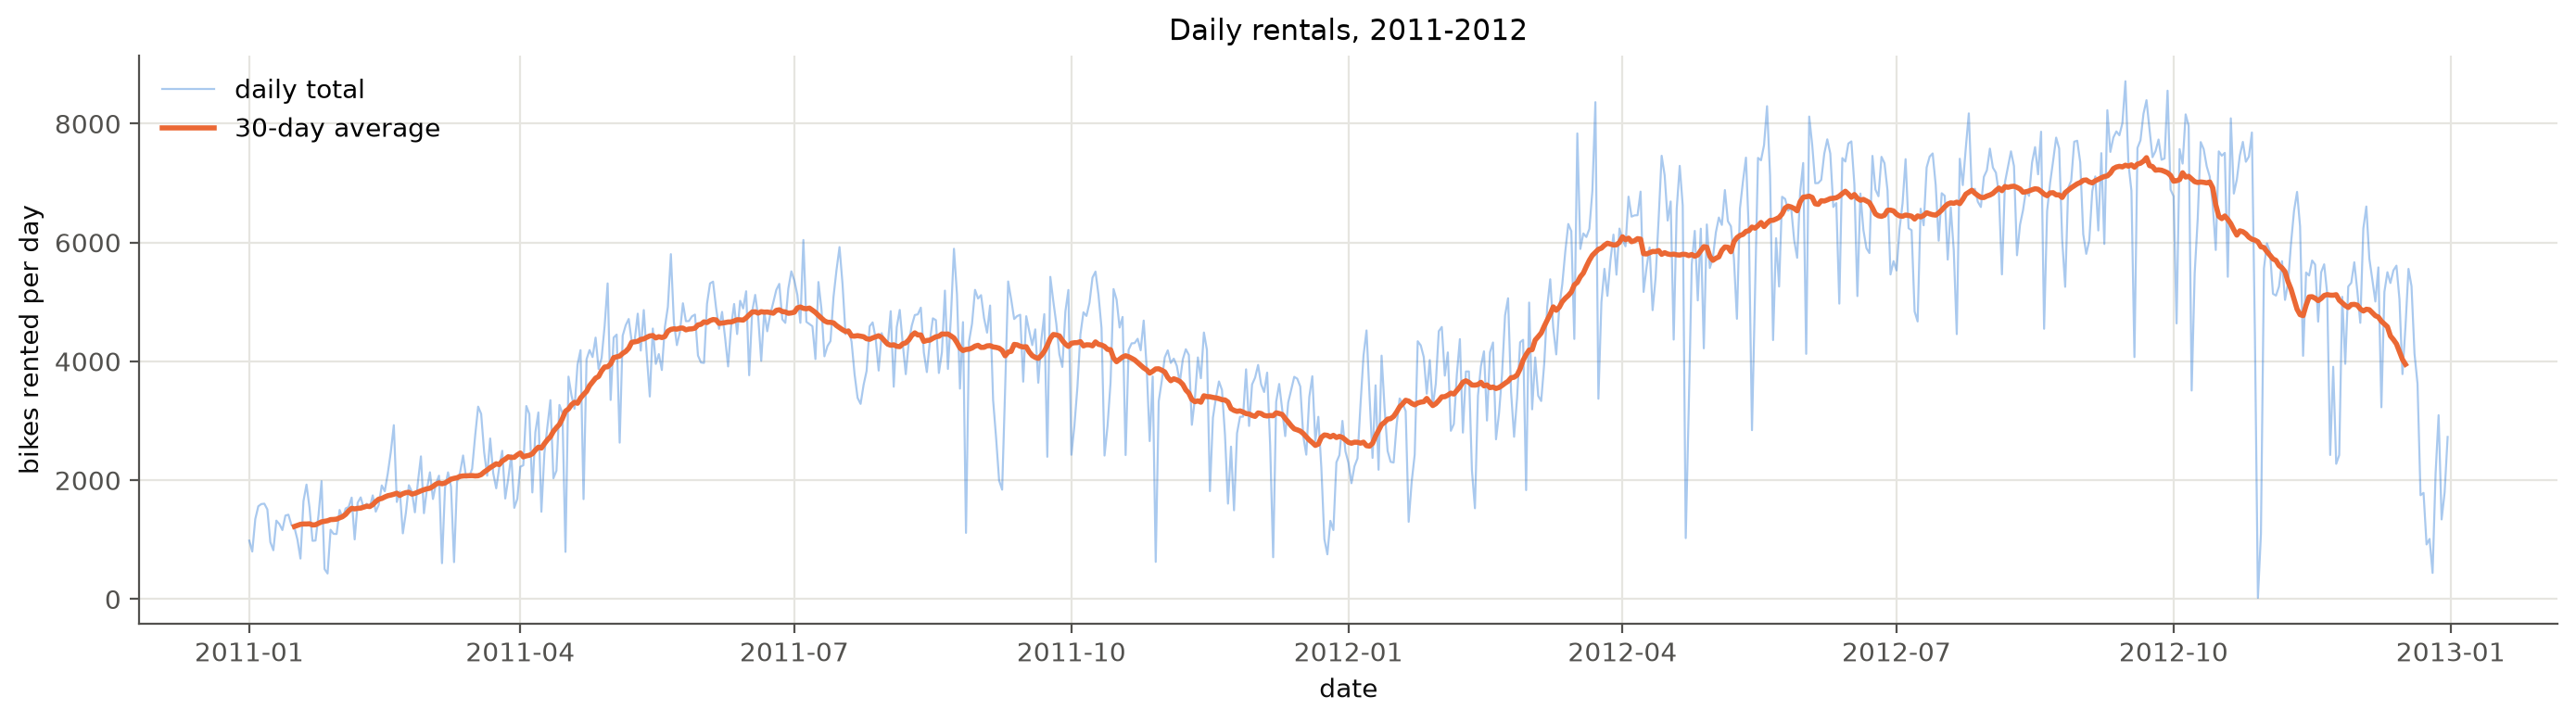
\includegraphics[width=\linewidth]{daily.png}
  \caption{Daily rentals over the two years: a yearly seasonal cycle and clear growth from 2011 to 2012.}
  \label{fig:daily}
\end{figure}

\begin{figure}[H]
  \centering
  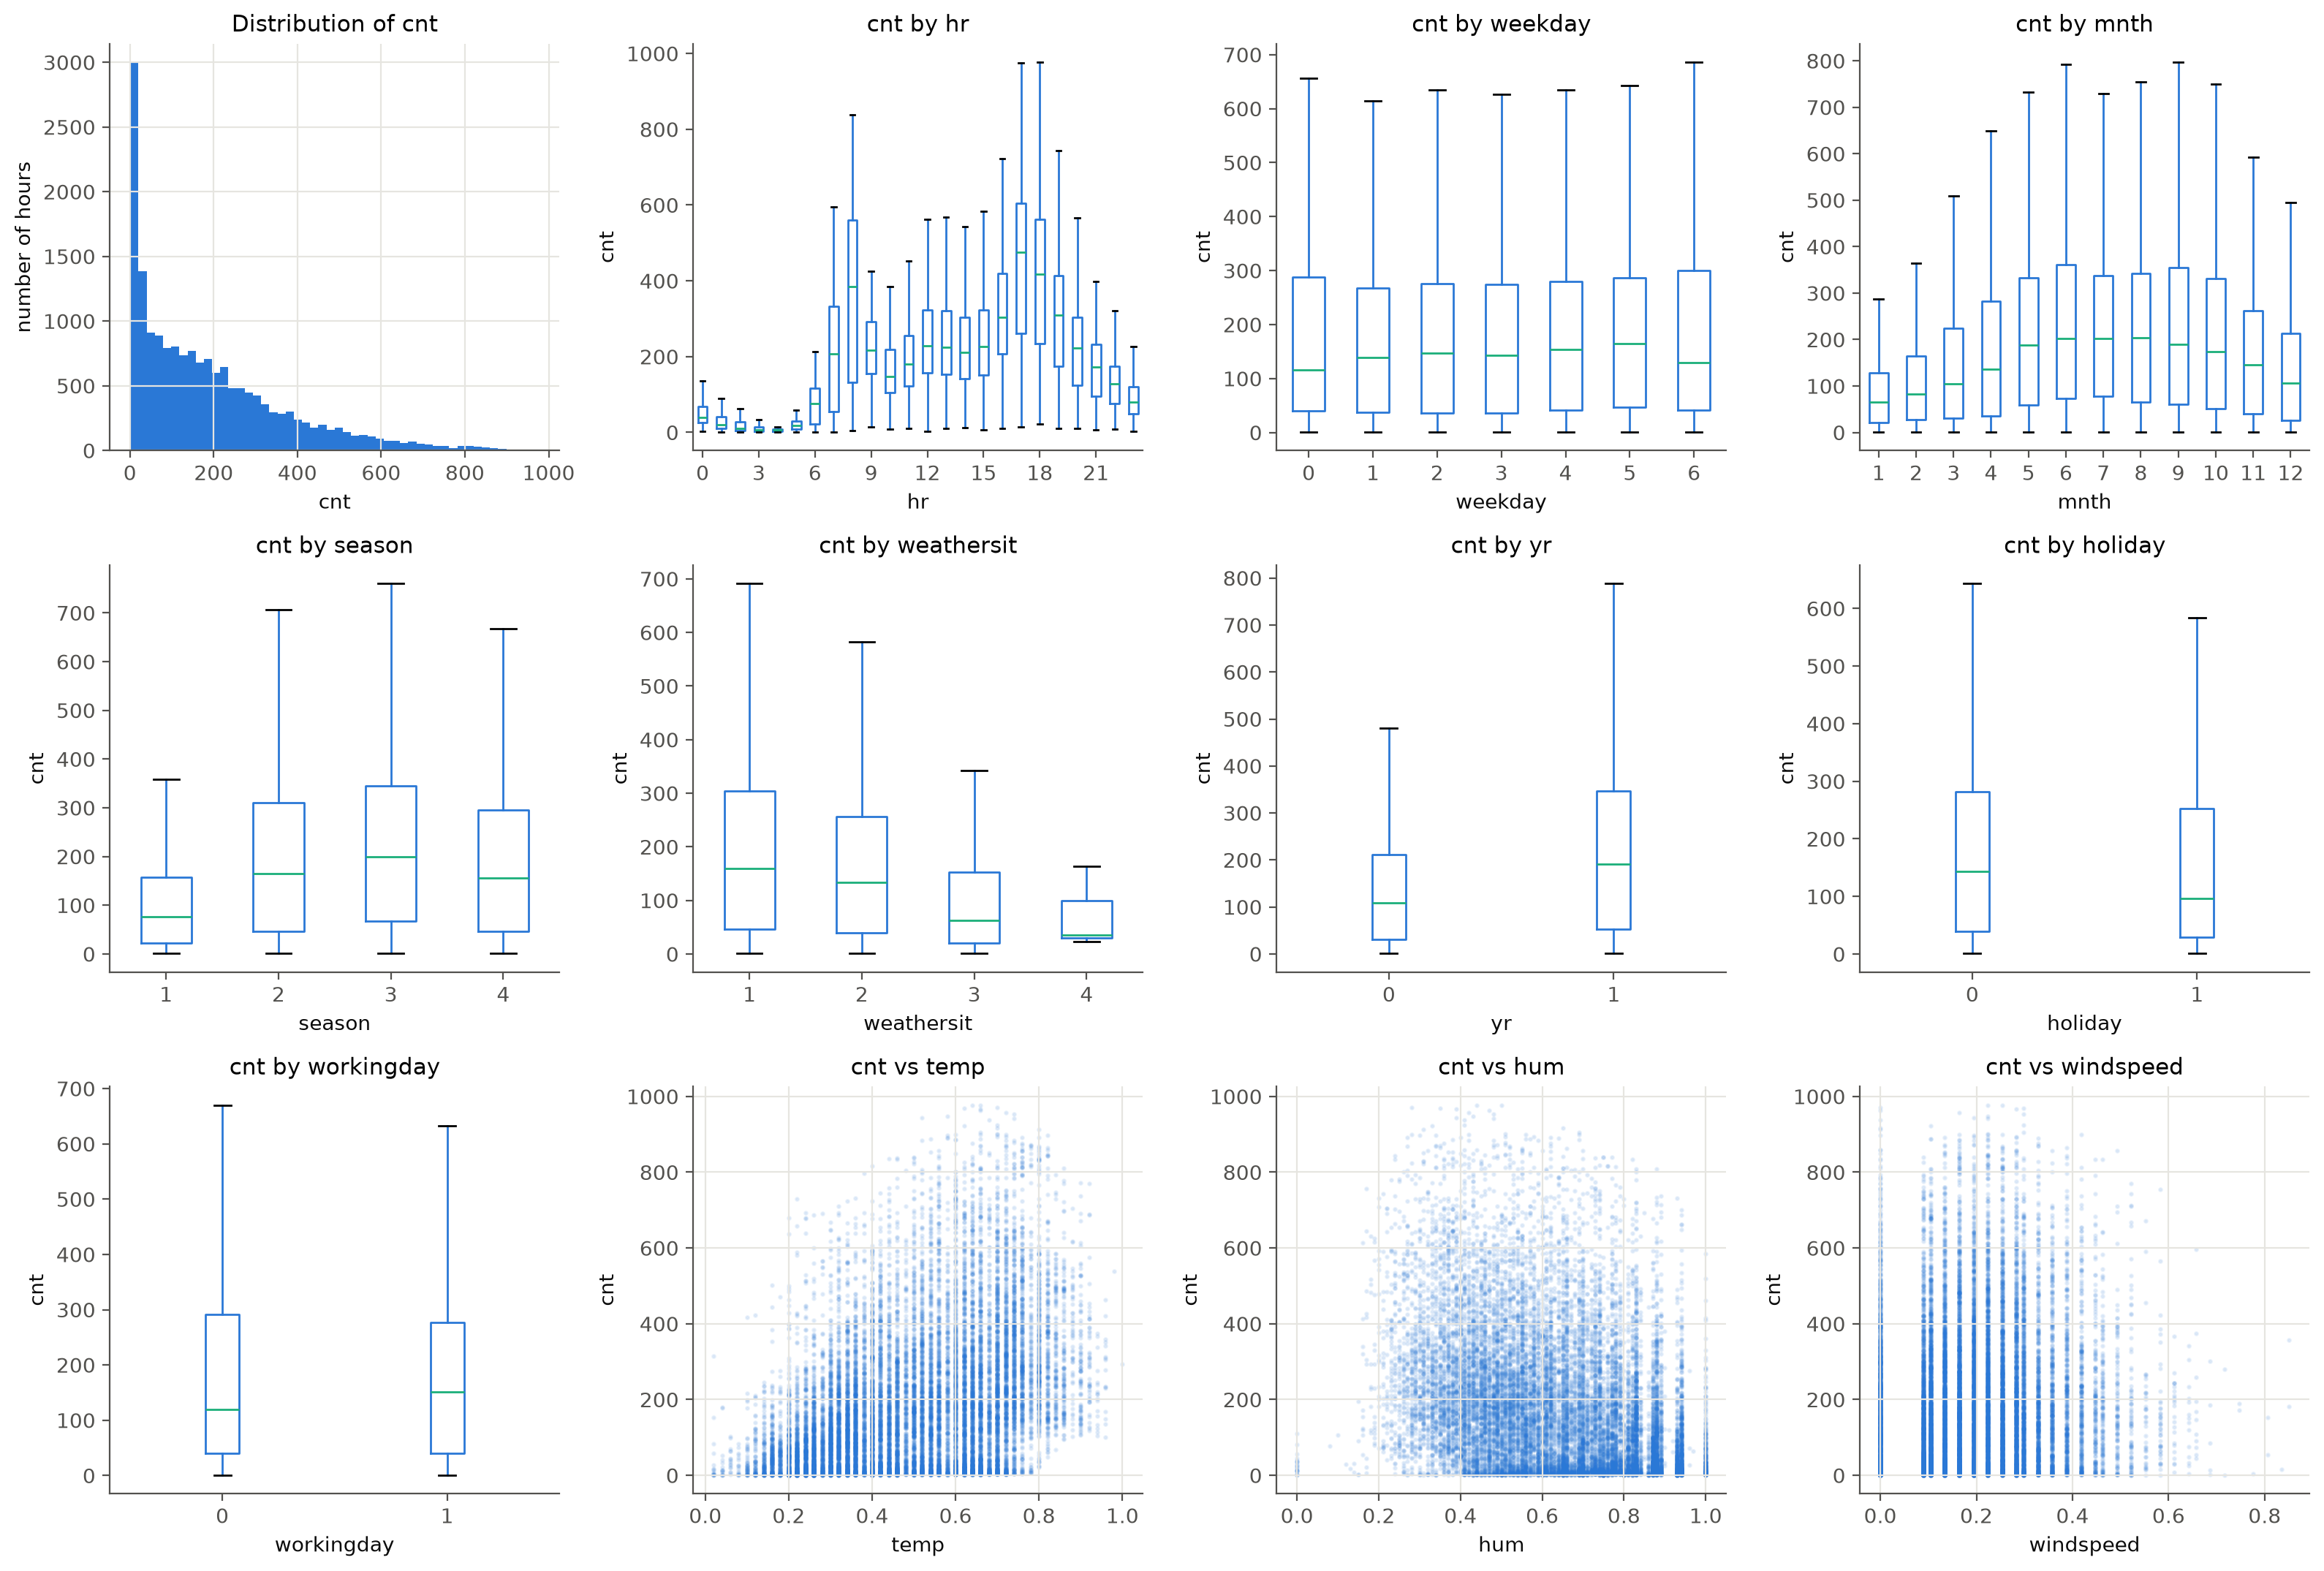
\includegraphics[width=\linewidth]{eda_grid.png}
  \caption{Distribution of \code{cnt} (top left), \code{cnt} against each categorical feature (box plots)
  and against each weather variable (scatter plots).}
  \label{fig:grid}
\end{figure}

\begin{figure}[H]
  \centering
  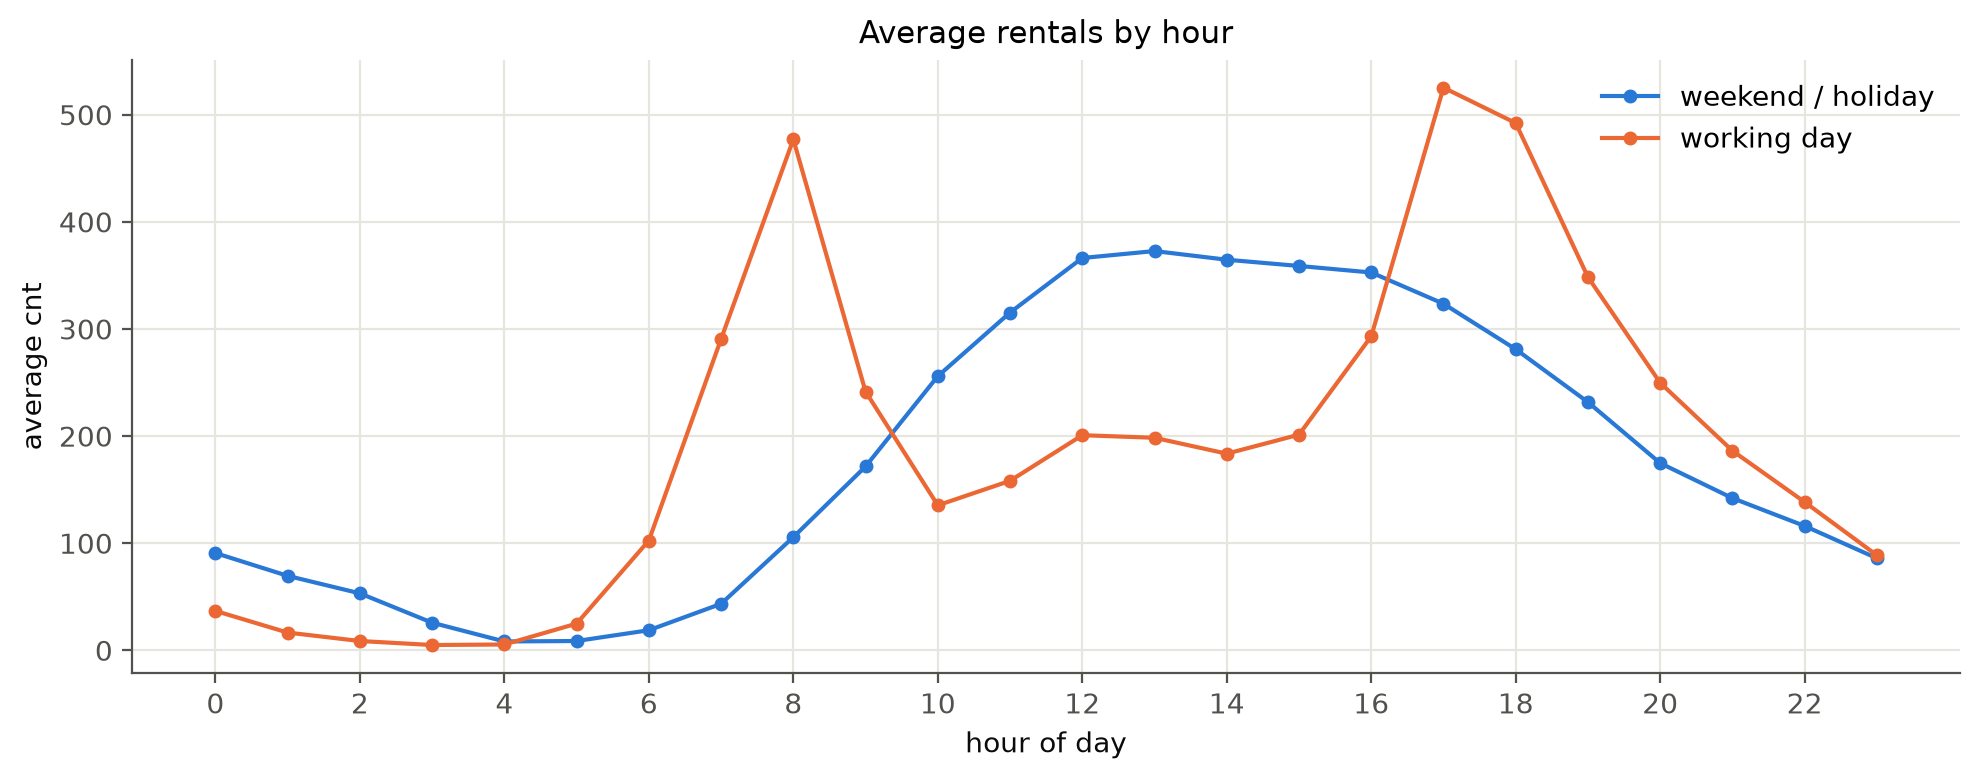
\includegraphics[width=0.85\linewidth]{hourly.png}
  \caption{Average rentals by hour, split by working day and weekend/holiday.}
  \label{fig:hourly}
\end{figure}

\begin{figure}[H]
  \centering
  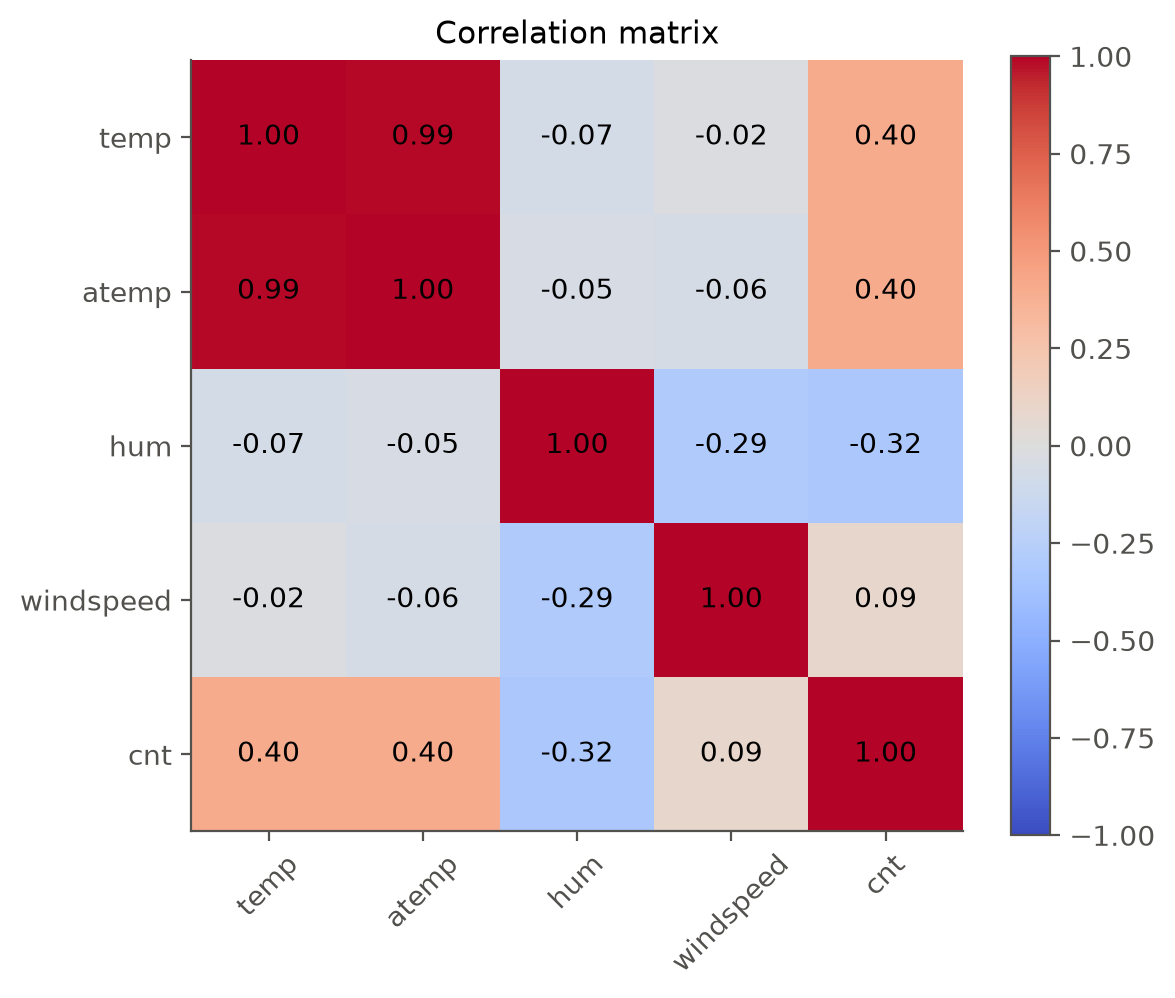
\includegraphics[width=0.55\linewidth]{corr.png}
  \caption{Correlation matrix of the continuous weather variables and \code{cnt}.}
  \label{fig:corr}
\end{figure}

\textbf{Interpretation.}
\begin{enumerate}
  \item \textbf{Trend and seasonality} (Figure~\ref{fig:daily}): rentals follow a yearly cycle, high in
        summer and low in winter, and 2012 is much busier than 2011, so \code{yr}, \code{season} and
        \code{mnth} should all matter.
  \item \textbf{The hour is the strongest pattern, and it depends on the type of day}
        (Figure~\ref{fig:hourly}). Working days have two commute peaks (477 bikes on average at 8:00 and 525 at 17:00);
        weekends and holidays have one midday hump (366 at 12:00, against 201 on working days).
        This is an \textbf{interaction} between \code{hr} and \code{workingday}, which a model that adds up
        feature effects separately cannot represent.
  \item \textbf{Non-linear and cyclical features:} a single weight on \code{hr} cannot follow two peaks,
        and hour 23 is next to hour 0 (and December next to January) even though the numbers are far apart.
  \item \textbf{Weather} (Figure~\ref{fig:corr}): \code{temp} has the strongest correlation with \code{cnt} (0.40),
        \code{hum} is negatively correlated ($-0.32$), and \code{windspeed} barely at all (0.09). Rentals drop as
        \code{weathersit} worsens. \code{temp} and \code{atemp} are almost identical (0.99).
  \item \textbf{\code{weekday} and \code{workingday} look unimportant in the box plots,} but this is misleading:
        working days and weekends peak at different hours, so their totals even out. The difference only
        appears hour by hour (point 2).
\end{enumerate}

% ===========================================================================
\section{Data Preparation}
% ===========================================================================

\textbf{Rationale.} Each issue found in Part 2 was handled with a decision justified by evidence
(Table~\ref{tab:prep}).

\begin{table}[H]
\centering
\caption{Data preparation decisions.}
\label{tab:prep}
\small
\begin{tabularx}{\linewidth}{@{}>{\raggedright\arraybackslash}p{2.4cm} >{\raggedright\arraybackslash}p{3.6cm} >{\raggedright\arraybackslash}p{2.6cm} X@{}}
\toprule
Issue & Evidence & Decision & Reason \\
\midrule
\code{dteday} is text & dtype \code{str} & Convert to datetime & Needed for time plots and the time-based split; not a model input. \\
Impossible humidity & 22 hours with \code{hum}$=0$, all on 2011-03-10 & Treat as missing; interpolate from neighbouring hours & The whole day is missing, so no same-day mean exists; humidity changes smoothly. \\
Rare category & \code{weathersit}~4 occurs 3 times & Merge into 3 & Too few examples to learn from; both are bad weather. \\
Redundant feature & corr(\code{temp}, \code{atemp}) $=0.988$; condition number of $X^TX$ is 216.8 with \code{atemp}, 12.9 without & Drop \code{atemp} & Near-duplicate columns make $X^TX$ close to singular, so the normal equation is unstable and the two weights trade off (multicollinearity). \\
Zero wind speed & 2,180 hours (12.5\%) exactly 0; next value 0.0896 & Keep & Calm cannot be told apart from a missing reading; imputing 1 in 8 rows would invent data, and \code{windspeed} later proves unimportant. \\
Missing hours & 17,544 expected, 17,379 present (165 missing) & Keep & Each hour is predicted from its own features, so gaps do not affect training. \\
Leakage & \code{casual} + \code{registered} $=$ \code{cnt} & Exclude & They contain the answer. \\
\bottomrule
\end{tabularx}
\end{table}

\textbf{Feature scaling.} Gradient descent, the polynomial models and Ridge use
\textbf{standardized} features (mean 0, standard deviation 1). For gradient descent this lets one
learning rate suit every weight; for Ridge, the penalty $\sum w_j^2$ is only fair if all features
are on the same scale. The scaler is always fitted on the training data only, so no information
from the validation or test set leaks into training. Plain least squares gives the same predictions
with or without scaling, and trees split on thresholds, so these use the raw features.

\textbf{Train / validation / test split.} A test set of 20\% (3,476 hours, \code{random\_state=42})
is set aside and used only for final results. The remaining 80\% is split again into a training set
(60\% overall, 10,427 hours) and a validation set (20\%, 3,476 hours), used to choose hyperparameters
(polynomial degree, $\lambda$, number of sine/cosine pairs). Choosing them on the test set would make
the test score optimistic. Once a hyperparameter is chosen, the final model is refitted on the full
80\%. A random split assumes the hours are \textbf{i.i.d.}; since neighbouring hours are strongly
related, Part 7 repeats the evaluation on a time-based split.

% ===========================================================================
\section{Initial Model: Multiple Linear Regression}
% ===========================================================================

\subsection{Rationale}

Linear regression is the natural baseline: it is the simplest regression model, fast and
interpretable, and its score sets the level every later model must beat. The hypothesis is
\begin{equation}
  \hat{y} = h(\x) = w_0 + w_1x_1 + \dots + w_{11}x_{11} = \w^T\x ,
  \qquad \hat{\y} = X\w \ \text{(vectorized)},
\end{equation}
with 12 parameters (11 weights and a bias). They minimize the cost~\eqref{eq:cost}, which can be done in two ways:
\begin{itemize}
  \item \textbf{Normal equation:} setting $\partial J/\partial\w = 0$ gives $\w = (X^TX)^{-1}X^T\y$
        (used by scikit-learn's \code{LinearRegression}~\cite{sklearn}).
  \item \textbf{Batch gradient descent:} start from $\w = \mathbf{0}$ and repeat
        $\w \leftarrow \w - \alpha \nabla J(\w)$, with $\nabla J(\w) = \frac{1}{N}X^T(X\w - \y)$ and learning rate $\alpha$.
        Implemented from scratch in NumPy to show the cost decreasing and to check that it reaches the same solution.
\end{itemize}
The coded features (\code{hr}, \code{season}, \code{weathersit}, \ldots) are used as plain numbers.
Part 2 already suggests this will underfit.

\subsection{Experiments and results}

\begin{figure}[H]
  \centering
  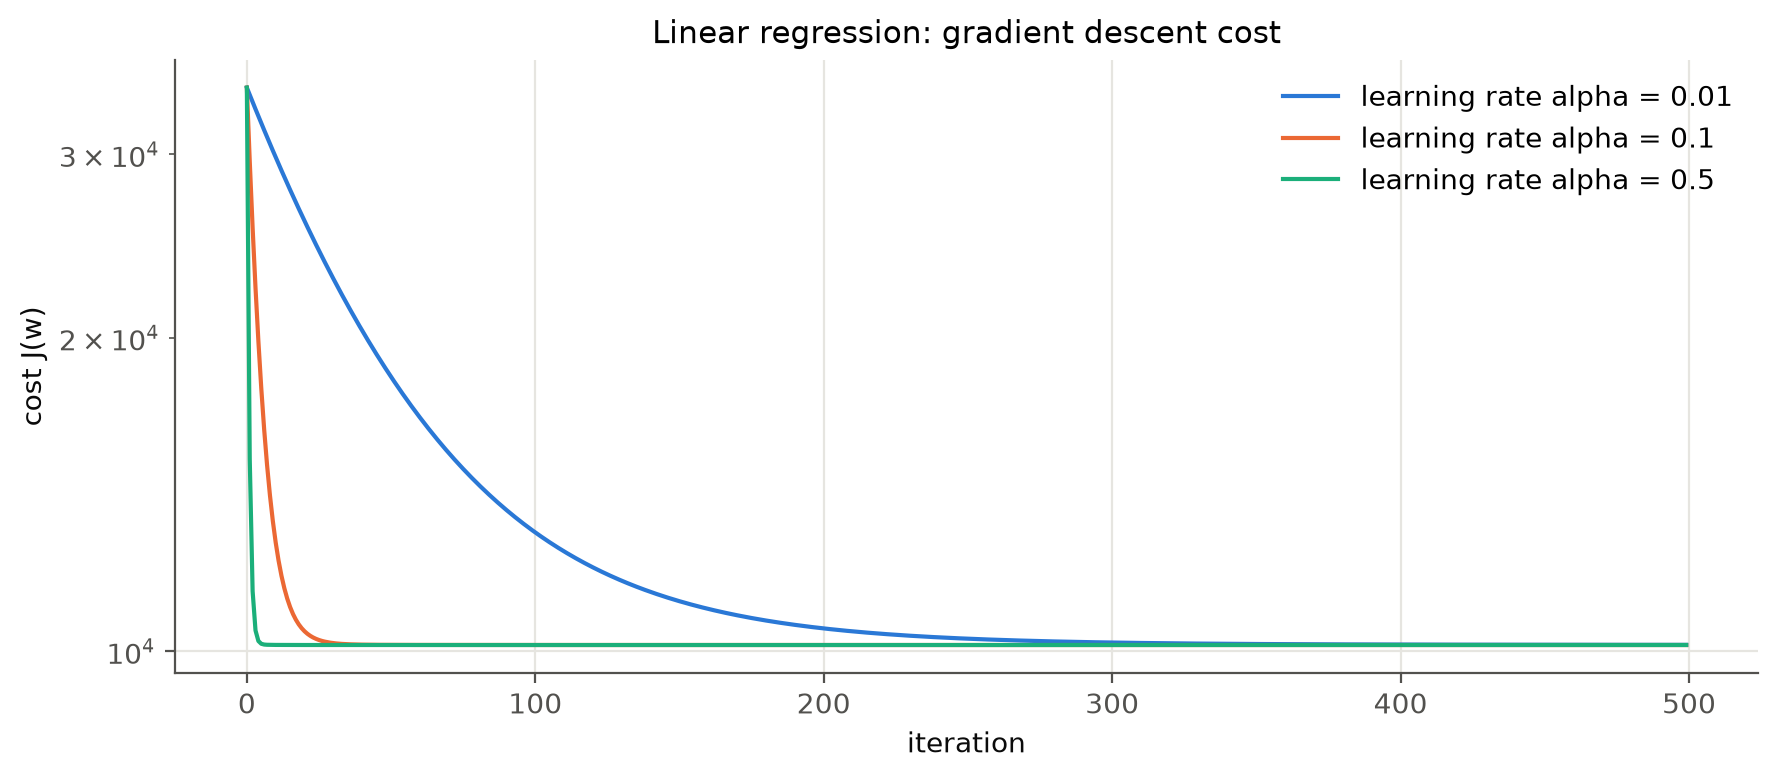
\includegraphics[width=0.8\linewidth]{gd.png}
  \caption{Gradient descent cost $J(\w)$ for three learning rates (log scale).}
  \label{fig:gd}
\end{figure}

\textbf{Gradient descent} (Figure~\ref{fig:gd}):
\begin{itemize}
  \item With $\alpha = 0.1$ the cost falls from 34,761 to its minimum of 10,136.1 within about 50
        iterations. The weights end within 0.0025 of the normal-equation solution, with the same test
        RMSE (139.3). Both methods reach the same minimum, as expected for a convex quadratic cost.
  \item $\alpha = 0.5$ converges in about 10 iterations and remains stable.
  \item $\alpha = 0.01$ is too small: after 500 iterations the cost is still 10,139.4 and some weights are 3.6 away from the solution.
  \item \textbf{Running more iterations does not overfit.} Training and test RMSE are unchanged from iteration 50
        to 5,000. Once the minimum of $J$ is reached, extra iterations change nothing; overfitting depends on the
        \emph{capacity} of the model (12 parameters, 10,427 examples), not on the number of iterations. Early stopping
        acts as regularization only for flexible models that can keep fitting noise (Section~\ref{sec:hgb}).
\end{itemize}

\begin{figure}[H]
  \centering
  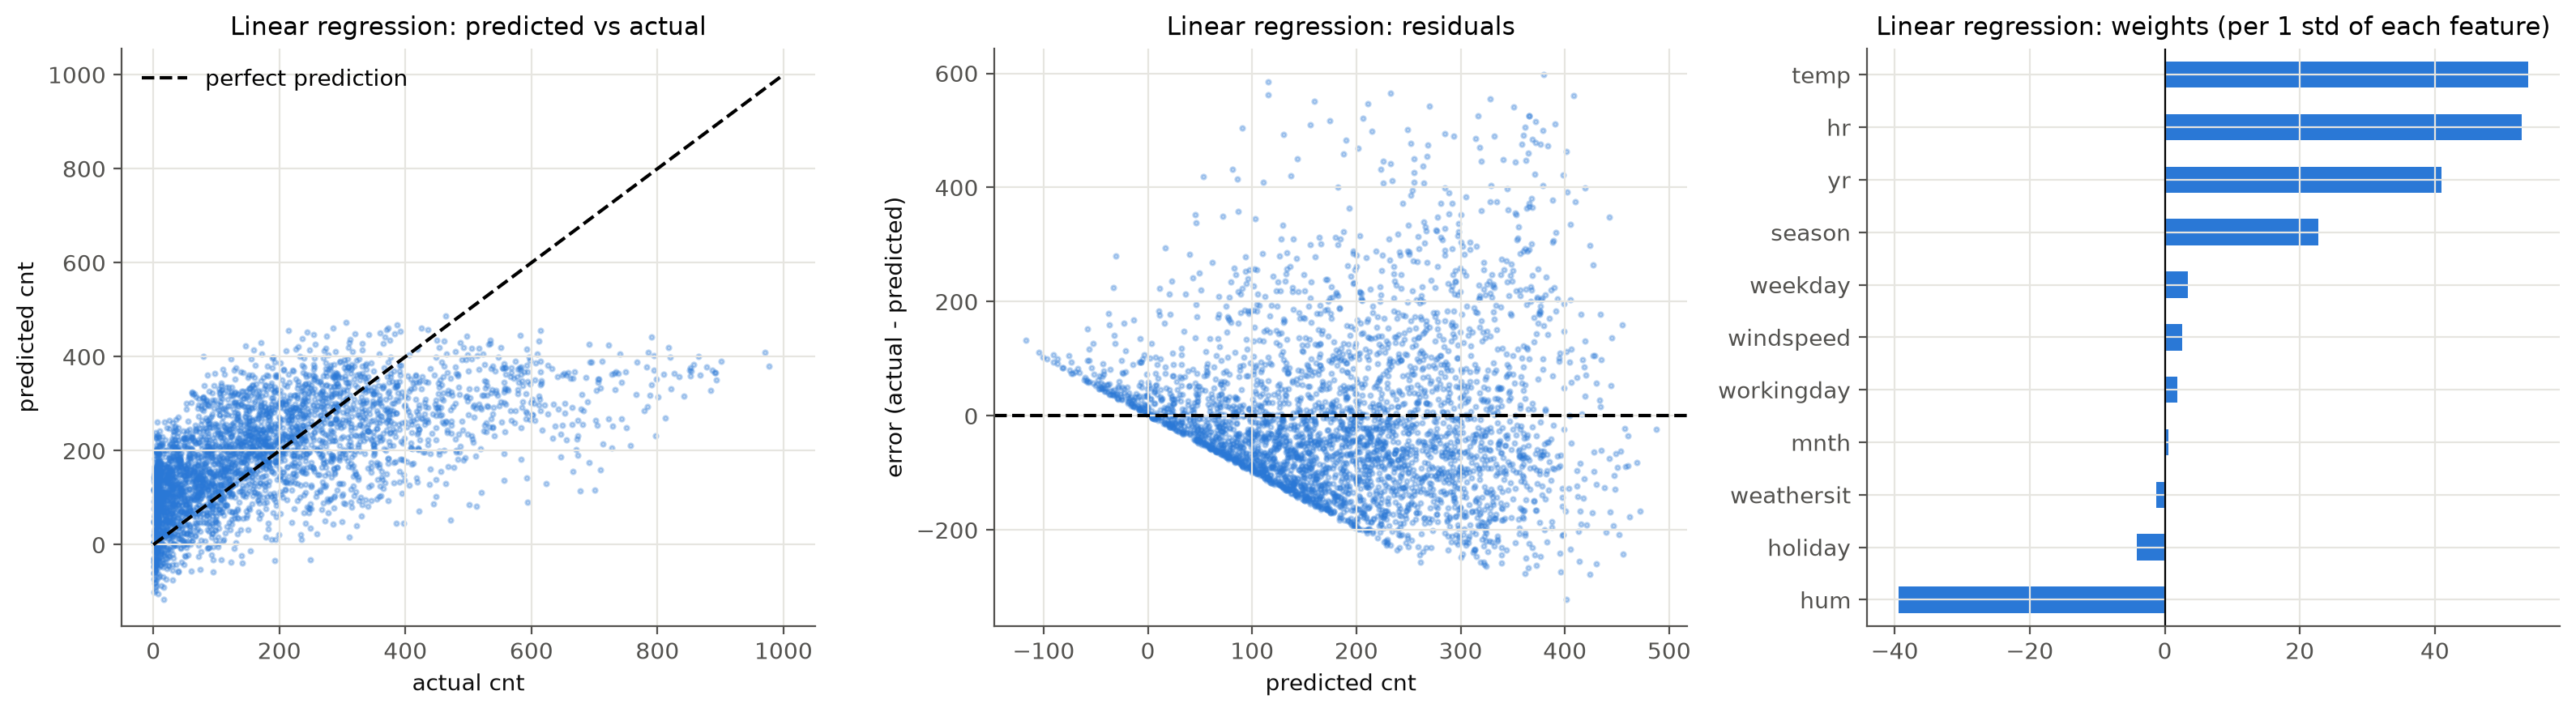
\includegraphics[width=\linewidth]{baseline.png}
  \caption{Linear regression baseline: predicted vs actual (left), residuals (centre), and weights per
  standard deviation of each feature (right).}
  \label{fig:baseline}
\end{figure}

\begin{table}[H]
\centering
\caption{Baseline results (random split).}
\label{tab:baseline}
\begin{tabular}{@{}lccc@{}}
\toprule
 & RMSE & MAE & $R^2$ \\
\midrule
Train & 142.4 & -- & 0.389 \\
Test  & 139.3 & 104.8 & 0.387 \\
\bottomrule
\end{tabular}
\end{table}

\subsection{Interpretation}

\begin{itemize}
  \item The baseline explains only 39\% of the variance, with an average error of 105 bikes when the average hour has 189.
  \item \textbf{Training and test errors are almost identical and both high}, so the model is
        \textbf{underfitting} (high bias): it is too simple for the pattern.
  \item Predictions never exceed 487, although up to 977 bikes were rented, and 158 test hours receive an
        impossible negative prediction. The residuals fan out as predictions grow, and 424 test hours are off by more than 200 bikes.
  \item \textbf{Weights} (Figure~\ref{fig:baseline}, right): \code{temp} ($+53.8$) and \code{hr} ($+52.8$) have the largest
        effect, followed by \code{yr} ($+41.0$) and \code{season} ($+22.7$); \code{hum} ($-39.5$) reduces rentals.
        \code{hr} gets one positive weight (``later means busier''), which cannot express two peaks.
        \code{weathersit}, \code{mnth} and \code{workingday} receive near-zero weights, not because they are unimportant,
        but because a single linear weight cannot capture their effect.
\end{itemize}

% ===========================================================================
\section{Model Complexity and Generalization}
% ===========================================================================

\textbf{Rationale.} Model complexity is the flexibility of the functions a model can fit, and
generalization is its ability to predict unseen data. Too little complexity causes
\textbf{underfitting} (high bias: training and validation error both high and close together);
too much causes \textbf{overfitting} (high variance: low training error, much higher validation error).
Three experiments examine this \textbf{bias--variance tradeoff}.

\subsection{Experiment 1: polynomial degree $M$}

Degree $M$ adds every product of the (standardized) features up to total degree $M$, giving a feature
map $\Psi(X)$. The model is still linear regression, now on $\Psi(X)$. Each degree is fitted on the
training set and scored on the validation set.

\begin{figure}[H]
  \centering
  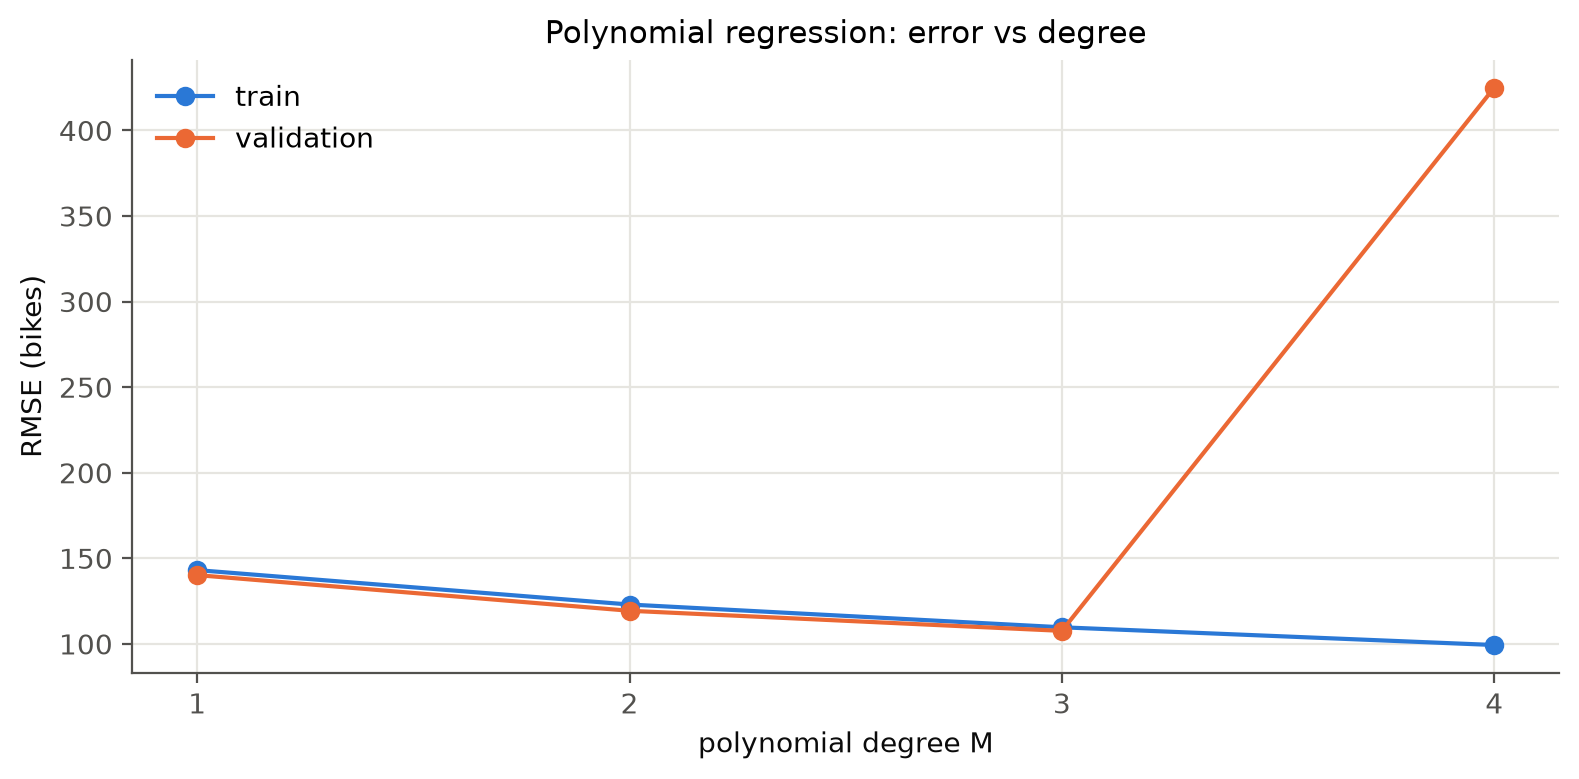
\includegraphics[width=0.72\linewidth]{degree.png}
  \caption{Training and validation RMSE against polynomial degree $M$.}
  \label{fig:degree}
\end{figure}

\begin{table}[H]
\centering
\caption{Polynomial degree experiment.}
\label{tab:degree}
\begin{tabular}{@{}ccccc@{}}
\toprule
$M$ & Columns & Train RMSE & Validation RMSE & Largest $|w|$ \\
\midrule
1 & 11    & 143.1 & 140.2 & 53 \\
2 & 77    & 123.0 & 119.4 & 64 \\
3 & 363   & 109.7 & 107.6 & 113 \\
4 & 1,364 & 99.4  & \textbf{425.0} & \textbf{3,207} \\
\bottomrule
\end{tabular}
\end{table}

\textbf{Interpretation.} From $M=1$ to 3 both errors fall together: added complexity reduces bias, but
the model still underfits. At $M=4$ the model \textbf{overfits}: training error keeps falling (99.4) while
validation error jumps to 425, worse than the baseline. The weights explode from at most 113 to 3,207,
so a small change in $\x$ causes a large change in $\hat{y}$. This motivates regularization (Part 6).

\subsection{Experiment 2: learning curve of the baseline}

\begin{figure}[H]
  \centering
  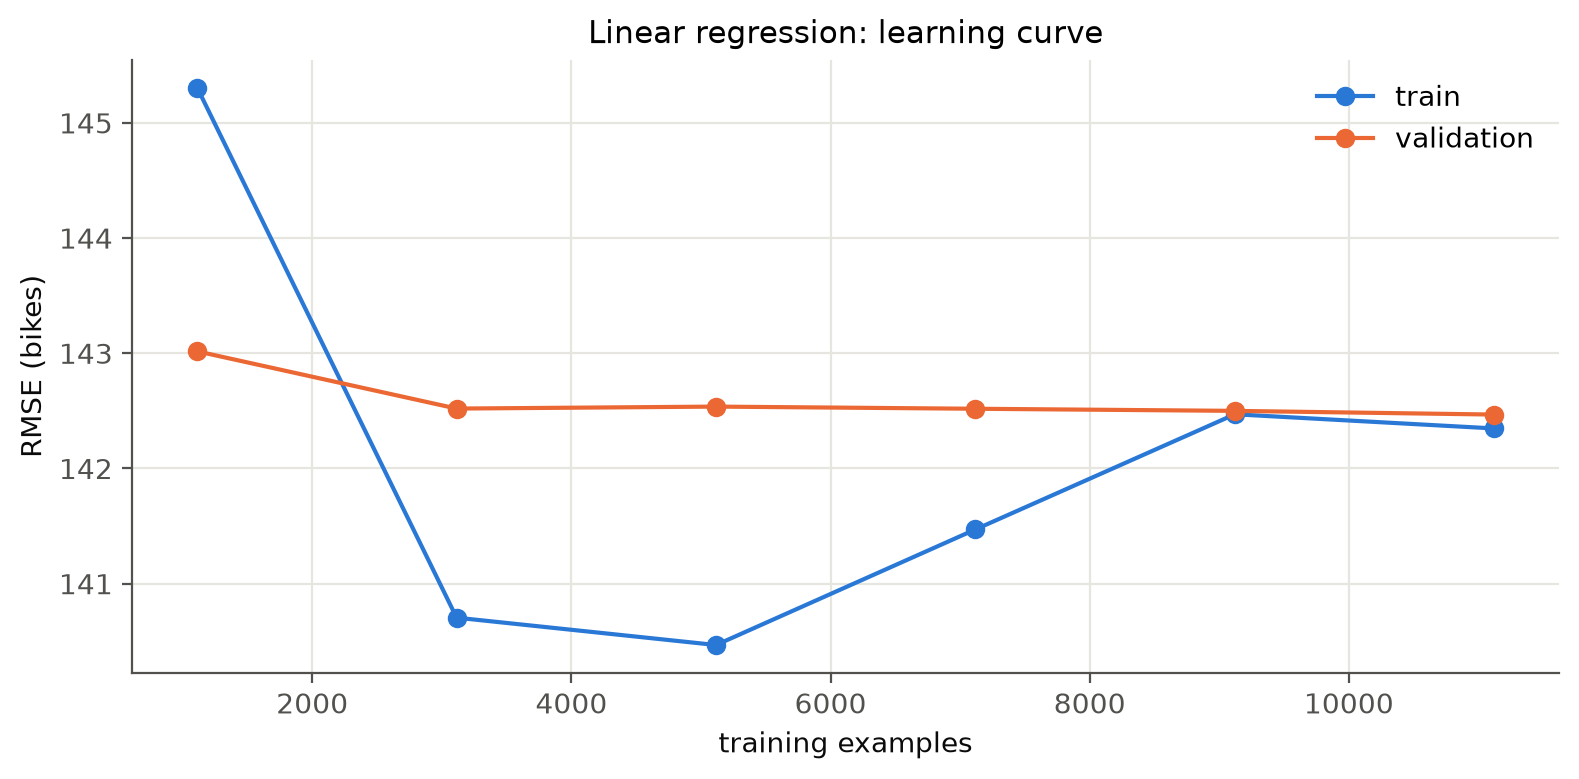
\includegraphics[width=0.72\linewidth]{lc_baseline.png}
  \caption{Learning curve of the linear baseline.}
  \label{fig:lc_baseline}
\end{figure}

From about 1,100 to 11,100 training examples, training and validation RMSE stay around 142 and
converge (142.3 and 142.5). Two curves that plateau close together at a high error are the signature
of \textbf{high bias}: more data will not help; the model needs more complexity or better features.

\subsection{Experiment 3: a more flexible model family (random forest)}

A random forest is an ensemble of decision trees built by \textbf{bagging}: each tree is trained on a
bootstrap sample of the training rows and the predictions are averaged. Trees split on thresholds
(e.g.\ \code{hr} $\le 7.5$), so they can follow any shape, learn interactions automatically (split on
\code{workingday}, then on \code{hr}) and need no scaling. The main model uses 200 full-depth trees.

\begin{figure}[H]
  \centering
  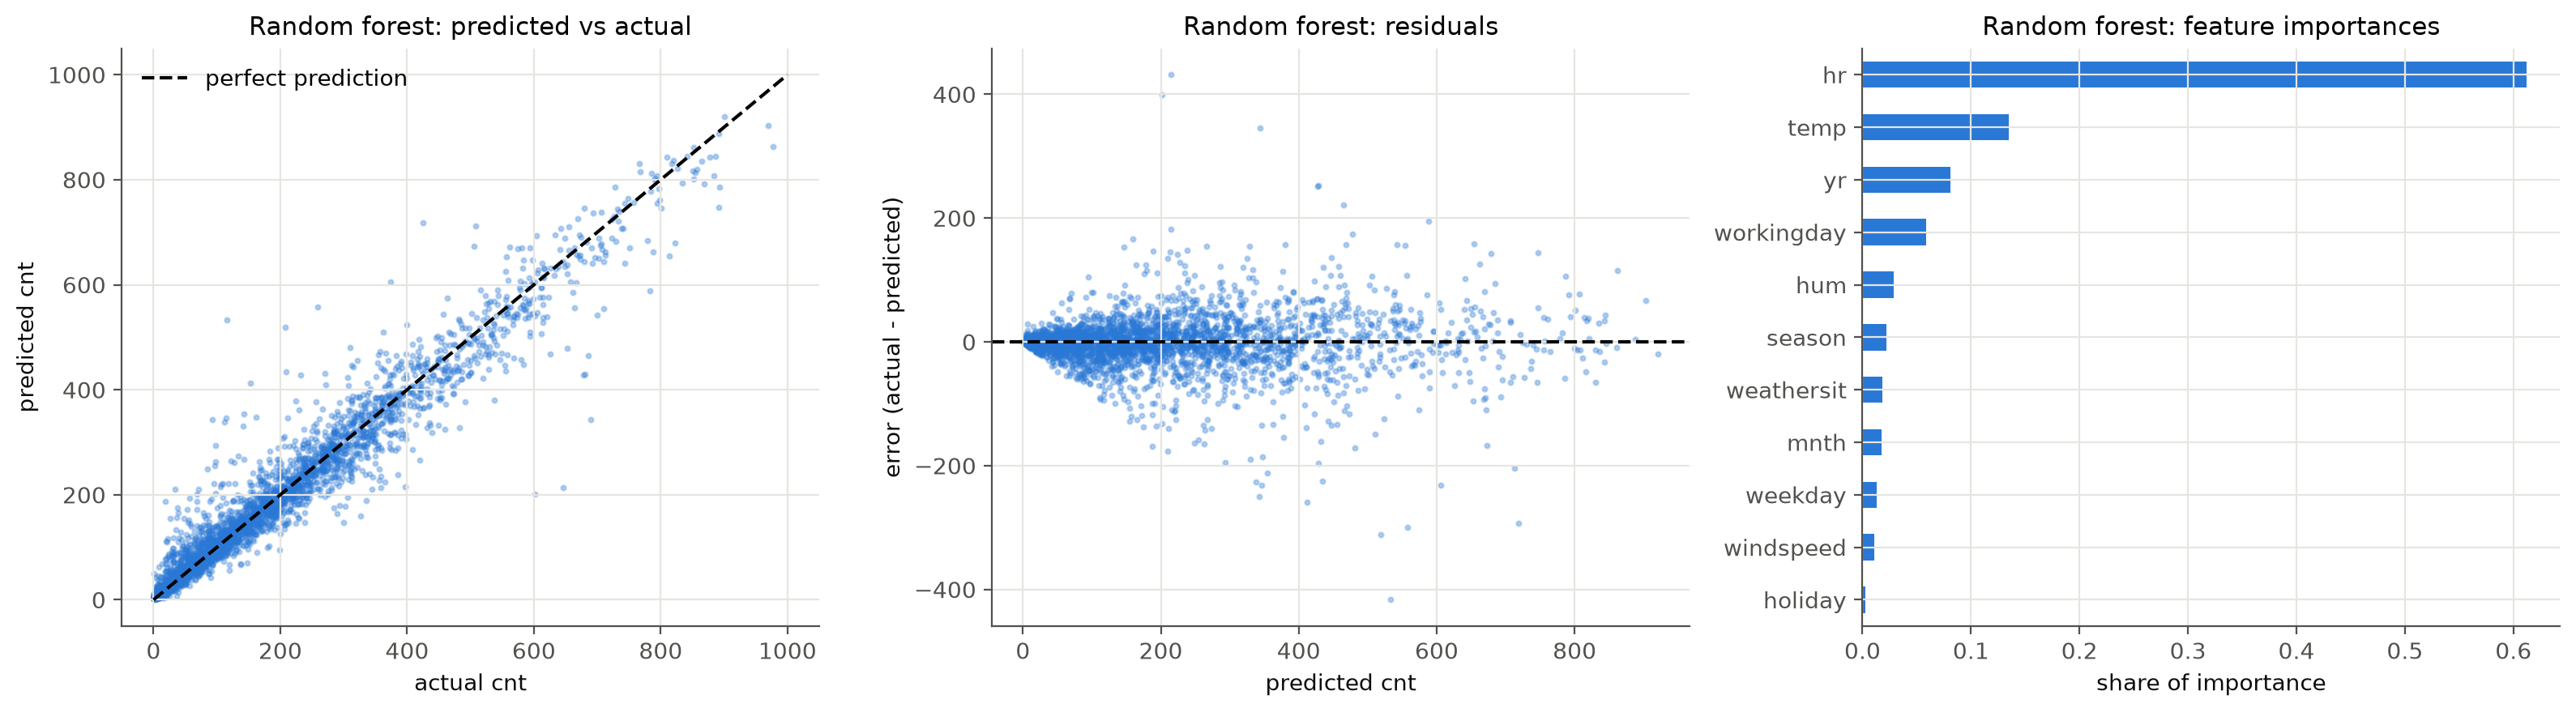
\includegraphics[width=\linewidth]{rf.png}
  \caption{Random forest: predicted vs actual, residuals and feature importances.}
  \label{fig:rf}
\end{figure}

\begin{itemize}
  \item \textbf{Test:} RMSE 42.0, MAE 24.6, $R^2 = 0.944$, less than a third of the baseline's error.
        Only 18 test hours are off by more than 200 bikes (424 for the baseline).
  \item \textbf{Train:} RMSE 15.9. The large train--test gap shows the trees \textbf{overfit}, yet they still generalize far better than the baseline.
  \item \textbf{Importances:} \code{hr} 0.61, \code{temp} 0.14, \code{yr} 0.08, \code{workingday} 0.06; \code{windspeed} only 0.01,
        which supports leaving its zero readings unchanged.
\end{itemize}

\begin{figure}[H]
  \centering
  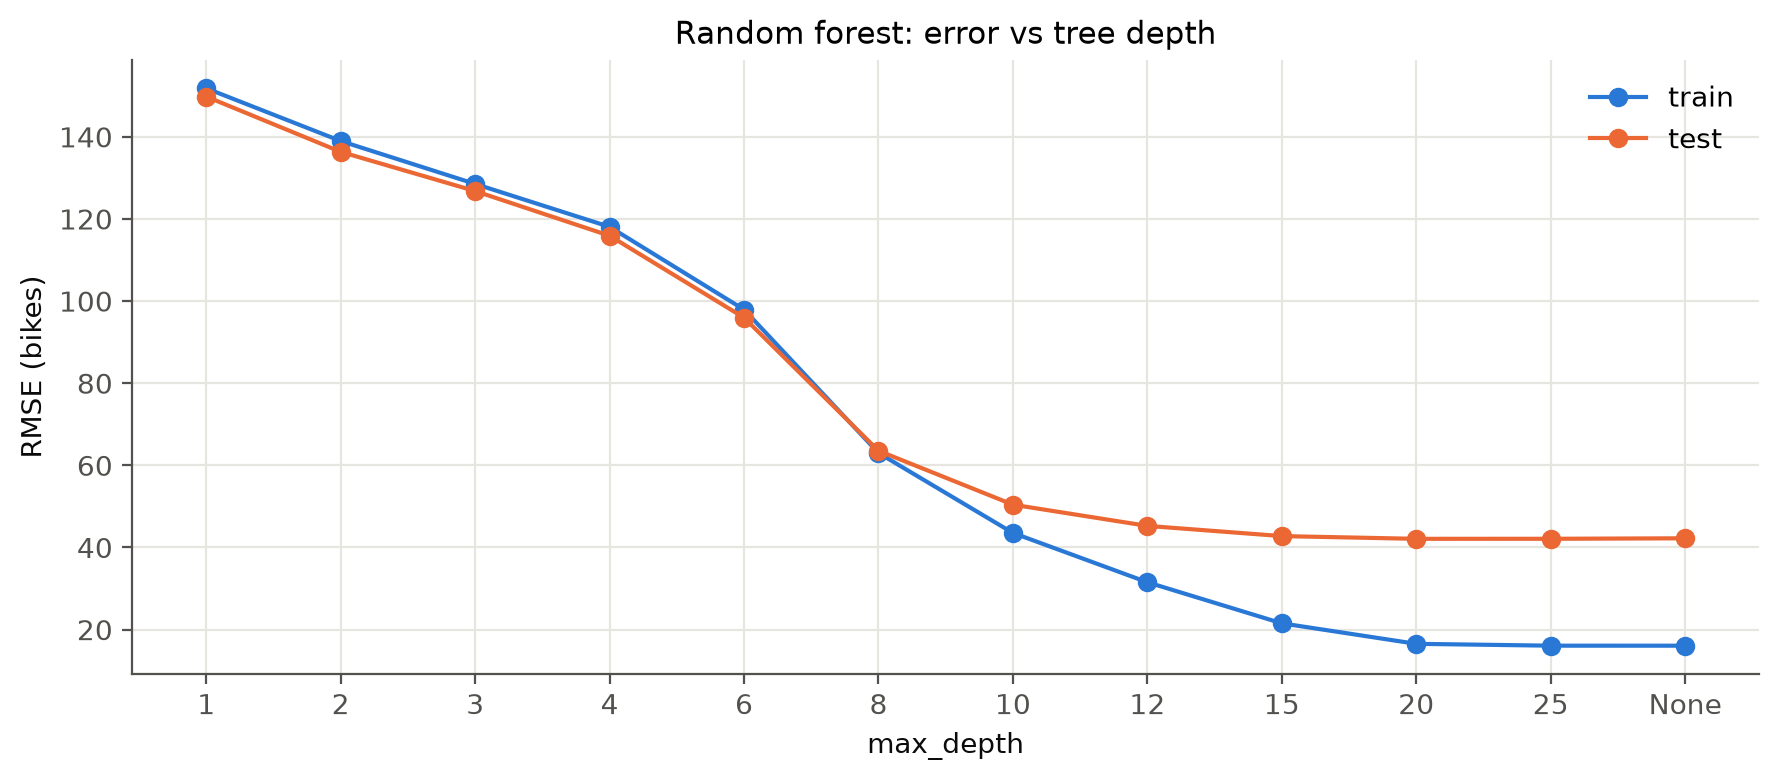
\includegraphics[width=0.72\linewidth]{depth.png}
  \caption{Random forest (100 trees) training and test RMSE against maximum tree depth.}
  \label{fig:depth}
\end{figure}

\textbf{Tree depth} (Figure~\ref{fig:depth}): at depths 1--6, training and test errors are equal and
high (about 150 down to 97): \textbf{underfitting}. Depth 8 balances the two (63.0 train, 63.5 test).
From depth 10 upward the training error keeps falling (to 16.1) while the test error levels off at
about 42; the gap grows to 26 bikes: \textbf{overfitting}. Unlike the polynomial model, test error does
\emph{not} rise again, because averaging many trees trained on different bootstrap samples cancels much
of each tree's variance. Depth therefore controls the bias--variance tradeoff, and bagging limits the
cost of high variance.

% ===========================================================================
\section{Improving the Model}
% ===========================================================================

\textbf{Rationale.} Part 5 found three problems: the linear baseline underfits, the degree-4
polynomial overfits with exploding weights, and the random forest has a 26-bike train--test gap.
Four remedies were applied: (1) regularization, (2) feature engineering, (3) gradient boosting with
early stopping, and (4) hyperparameter tuning with cross-validation.

\subsection{Regularization: Ridge regression}

Ridge (L2) regression keeps the complex degree-4 model but penalizes large weights:
\begin{equation}
  J(\w) = \frac{1}{2N}\sum_{i=1}^{N}\left(y^{(i)} - \hat{y}^{(i)}\right)^2 + \frac{\lambda}{2N}\sum_{j} w_j^2 .
\end{equation}
$\lambda = 0$ recovers the overfitting model, while a very large $\lambda$ shrinks all weights towards
0 and underfits. $\lambda$ is a \textbf{hyperparameter}: candidates in powers of ten were each scored on
the validation set and the lowest validation error was kept. L2 was preferred over L1 (Lasso) because
the goal is to shrink 1,364 correlated terms smoothly rather than select a few.

\begin{figure}[H]
  \centering
  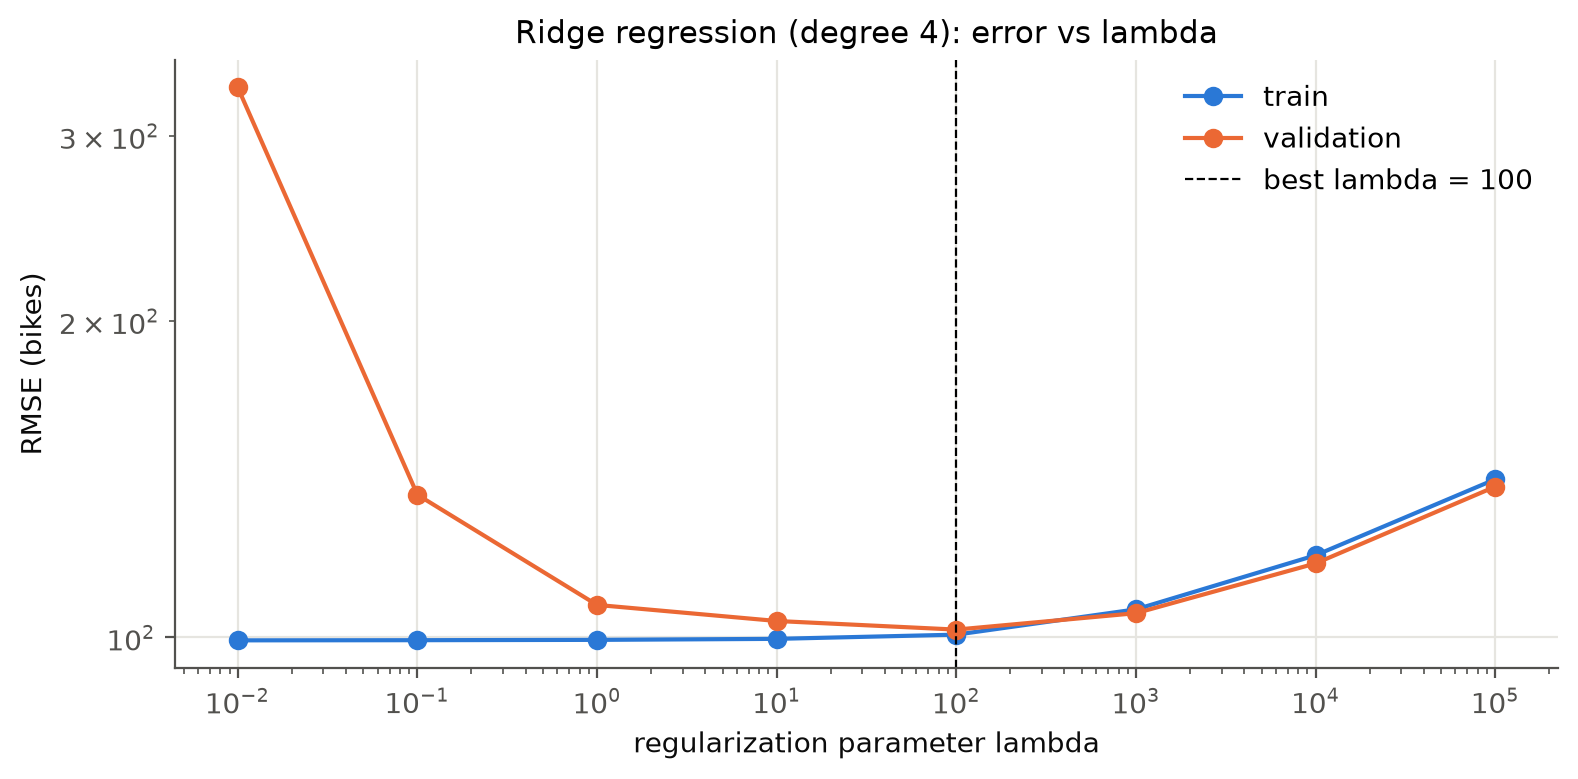
\includegraphics[width=0.72\linewidth]{ridge.png}
  \caption{Ridge regression on degree-4 features: training and validation RMSE against $\lambda$.}
  \label{fig:ridge}
\end{figure}

\begin{table}[H]
\centering
\caption{Ridge regularization path (degree 4).}
\label{tab:ridge}
\begin{tabular}{@{}lccc@{}}
\toprule
$\lambda$ & Train RMSE & Validation RMSE & Largest $|w|$ \\
\midrule
0 (no regularization) & 99.4 & 425.0 & 3,207 \\
0.01    & 99.4  & 333.6 & 609 \\
0.1     & 99.4  & 136.7 & 253 \\
1       & 99.5  & 107.4 & 126 \\
10      & 99.7  & 103.7 & 124 \\
\textbf{100} & \textbf{100.6} & \textbf{101.7} & \textbf{105} \\
1,000   & 106.3 & 105.5 & 46 \\
10,000  & 119.7 & 117.6 & 12 \\
100,000 & 141.4 & 139.1 & 4 \\
\bottomrule
\end{tabular}
\end{table}

\textbf{Interpretation.} The validation error is U-shaped in $\lambda$: too little regularization overfits,
too much underfits (139.1 at $\lambda=10^5$, about the baseline). At $\lambda = 100$ the largest weight shrinks
from 3,207 to 105 and the train--validation gap closes from 326 bikes to about 1. Refitted on the full
80\%, the test result is RMSE 102.2, MAE 71.9, $R^2 = 0.670$, a large improvement on the baseline.
Limitations remain: 190 negative test predictions, and close, still-high errors (train 99.9, test 102.2),
so the model has moved back to mild underfitting. Smooth polynomials cannot follow the sharp commute peaks.

\subsection{Feature engineering: sinusoidal features}

Instead of thousands of generic polynomial terms, a few features were designed from the exploration:
\begin{itemize}
  \item \textbf{Sine/cosine (Fourier) basis functions of the hour}, for $k = 1,\dots,K$:
        \[
          \text{hr\_sin}_k = \sin\!\left(\tfrac{2\pi k\,\text{hr}}{24}\right), \qquad
          \text{hr\_cos}_k = \cos\!\left(\tfrac{2\pi k\,\text{hr}}{24}\right).
        \]
        The model stays linear in its parameters but can fit a smooth, repeating daily curve in which 23:00 sits
        next to 0:00. \code{mnth} gets one sine/cosine pair with a 12-month period.
  \item \textbf{Interaction with \code{workingday}:} each hour wave is also multiplied by \code{workingday},
        so working days get their own daily curve (the commute peaks).
  \item \textbf{Log target:} the model is trained on $\log(\text{cnt}+1)$ and predictions are transformed back with
        $e^{z}-1$. This reduces skew, suits multiplicative effects (rain cuts rentals by a percentage), and
        guarantees positive predictions.
\end{itemize}
$K$ was chosen on the validation set as the smallest $K$ within one bike of the best validation error
(prefer the simpler model when extra complexity gains almost nothing).

\begin{figure}[H]
  \centering
  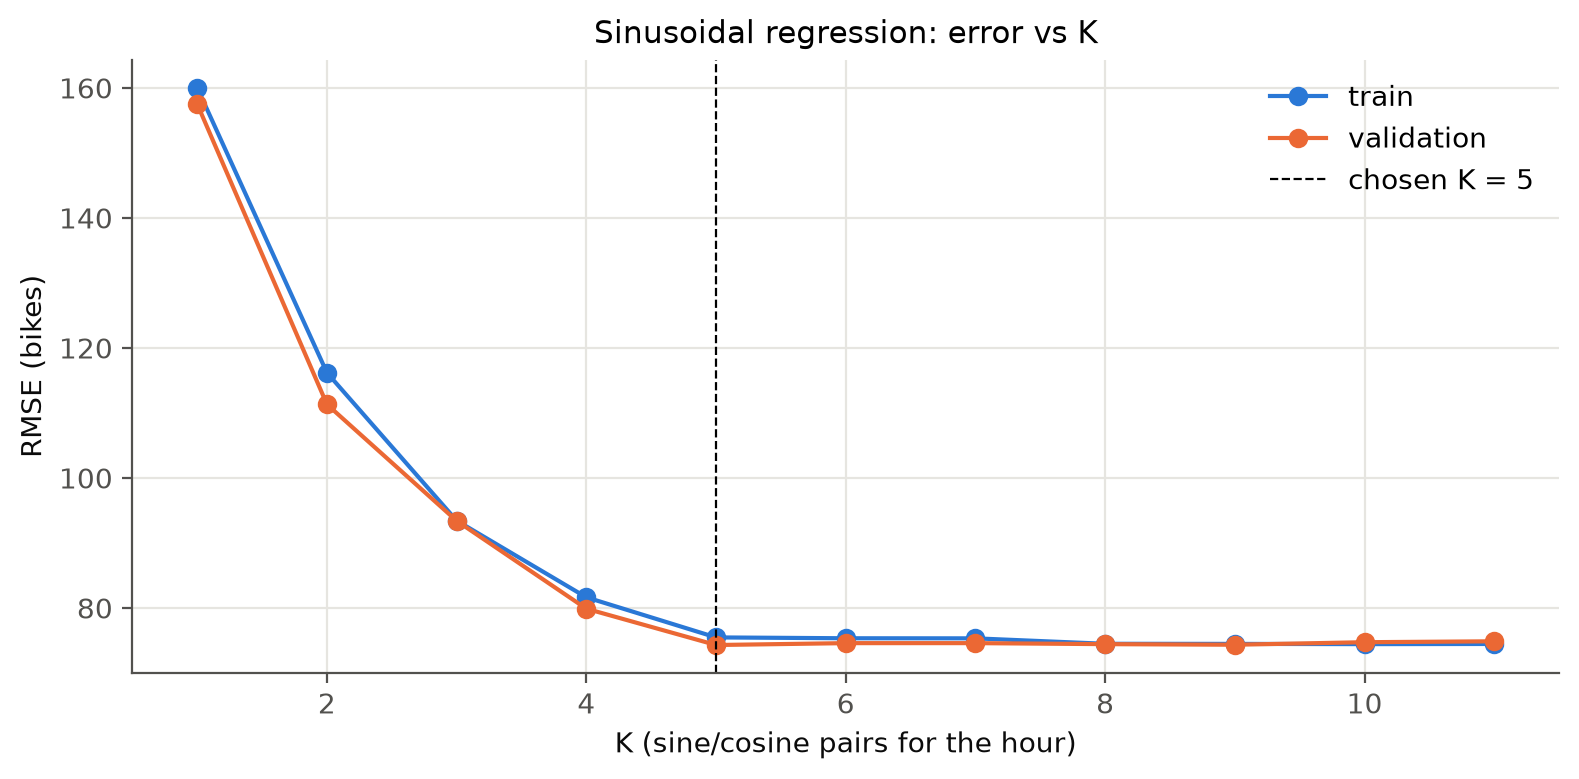
\includegraphics[width=0.72\linewidth]{sin_K.png}
  \caption{Training and validation RMSE against the number of sine/cosine pairs $K$.}
  \label{fig:sinK}
\end{figure}

$K=1$ underfits (RMSE 160.0 train, 157.5 validation): one wave per day cannot produce two peaks.
The error falls steadily (93.4 at $K=3$, 79.9 at $K=4$) and levels off at about 74--75 from $K=5$
(validation 74.3), which was chosen (31 columns). Train and validation curves stay within 5 bikes of
each other at every $K$, so there is no overfitting.

\begin{figure}[H]
  \centering
  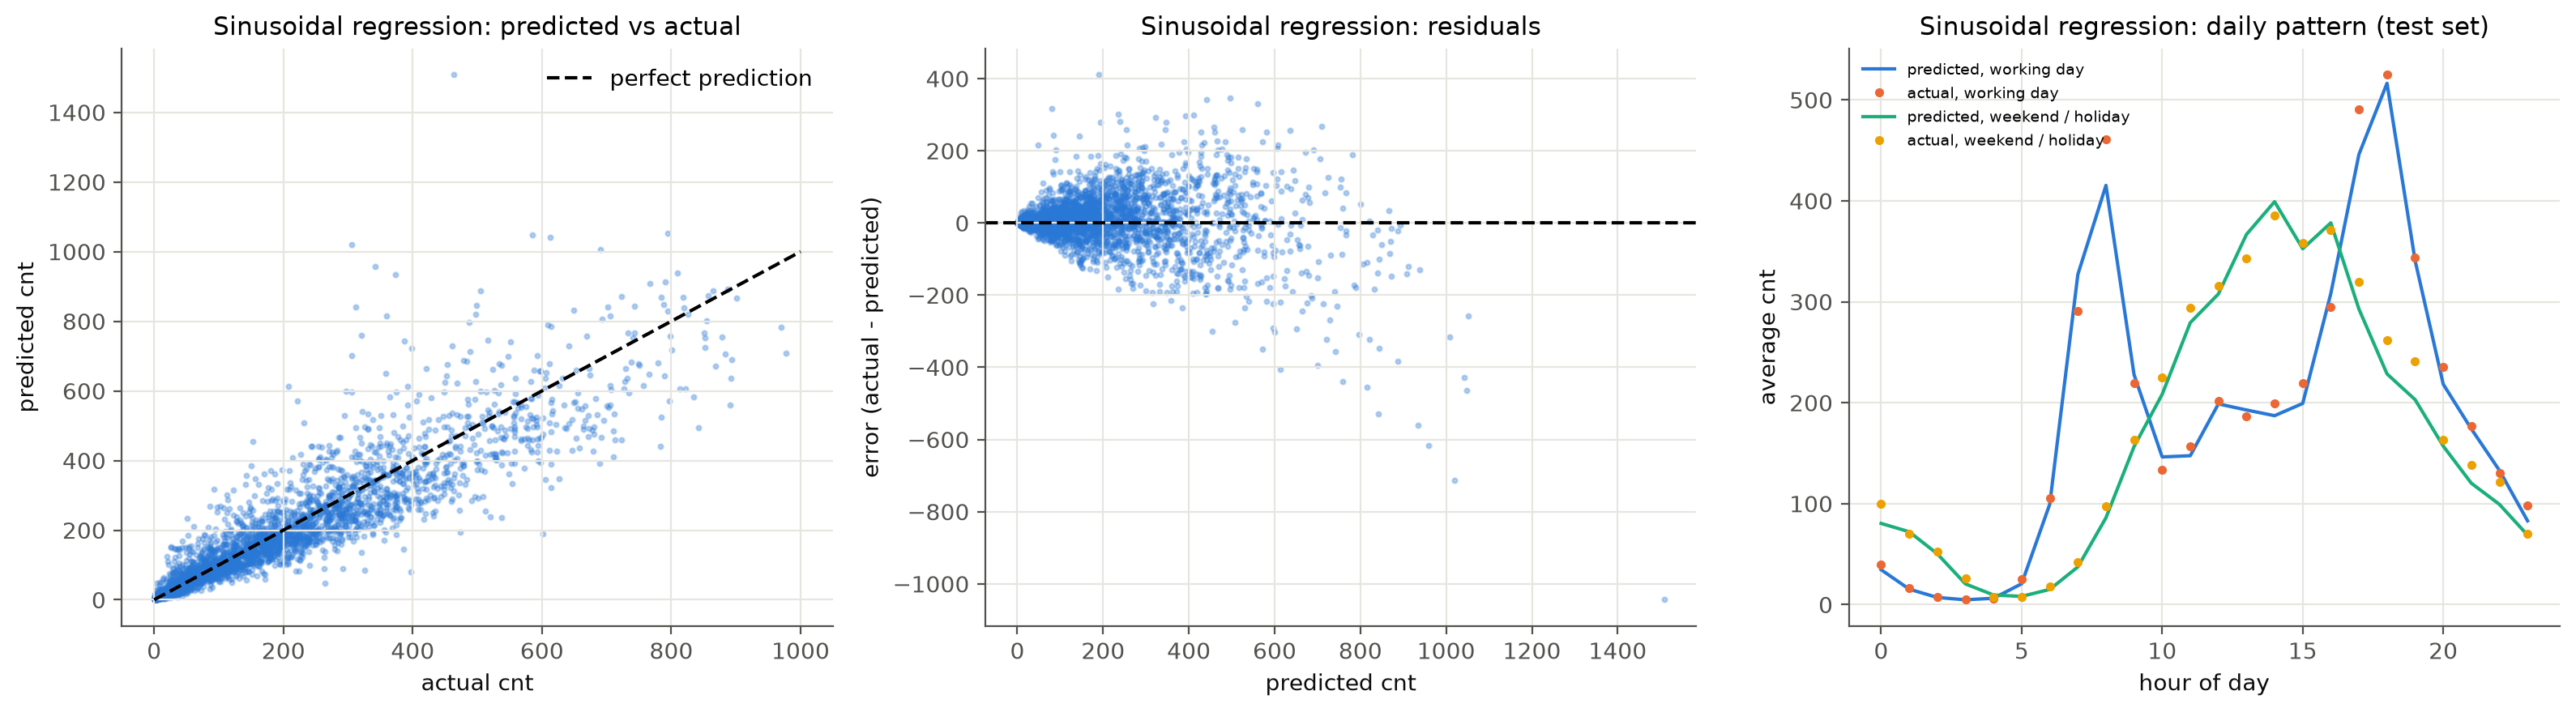
\includegraphics[width=\linewidth]{sin.png}
  \caption{Sinusoidal regression ($K=5$): predicted vs actual, residuals, and average daily pattern on the test set.}
  \label{fig:sin}
\end{figure}

\textbf{Results.} Test RMSE 75.1, MAE 43.8, $R^2 = 0.822$ (train RMSE 74.6, $R^2 = 0.832$). With only 20
extra columns the error is almost halved compared with the baseline, and the model beats the
regularized degree-4 polynomial (102.2) with 1,333 fewer columns: \emph{better features beat more features}.
Train and test errors are almost identical, so the remaining error is bias. The daily-pattern panel shows
the commute peaks are still smoothed (8:00 on working days: 415 predicted vs 461 actual; 17:00: 446 vs 491),
while weekends fit well (14:00: 399 vs 385). Only 83 test hours are off by more than 200 bikes, but a few
predictions overshoot badly (up to 1,508): a modest error on the log scale becomes large after exponentiation.

\subsection{Gradient boosting with early stopping}
\label{sec:hgb}

\textbf{Boosting} builds small trees sequentially; each new tree is fitted to the errors the current
ensemble still makes (for squared error, the negative gradient of the loss is the residual), scaled by a
learning rate. Bagging reduces variance by averaging independent trees; boosting reduces bias step by
step, in effect performing gradient descent in function space. \code{HistGradientBoostingRegressor}
bins each feature into at most 255 values for speed; it was used with up to 63 leaves per tree and up to
500 trees. \textbf{Early stopping} acts as regularization: 10\% of the training data is held out, and
training stops when the validation loss has not improved for 10 iterations.

\begin{figure}[H]
  \centering
  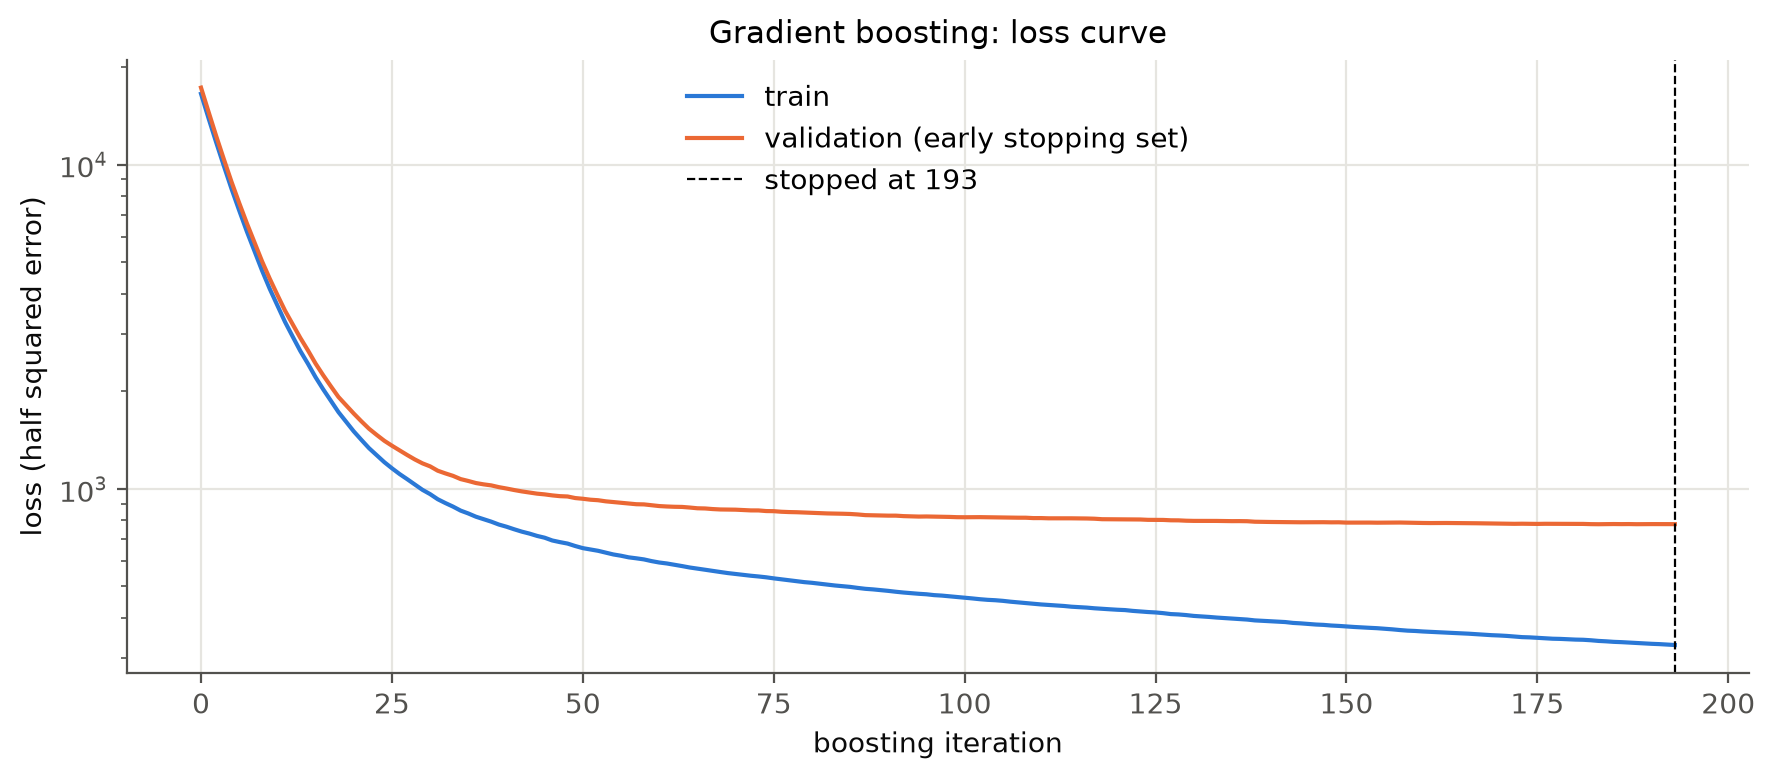
\includegraphics[width=0.72\linewidth]{hgb_loss.png}
  \caption{Gradient boosting training and validation loss per iteration (training stopped early at iteration 193).}
  \label{fig:hgbloss}
\end{figure}

\begin{figure}[H]
  \centering
  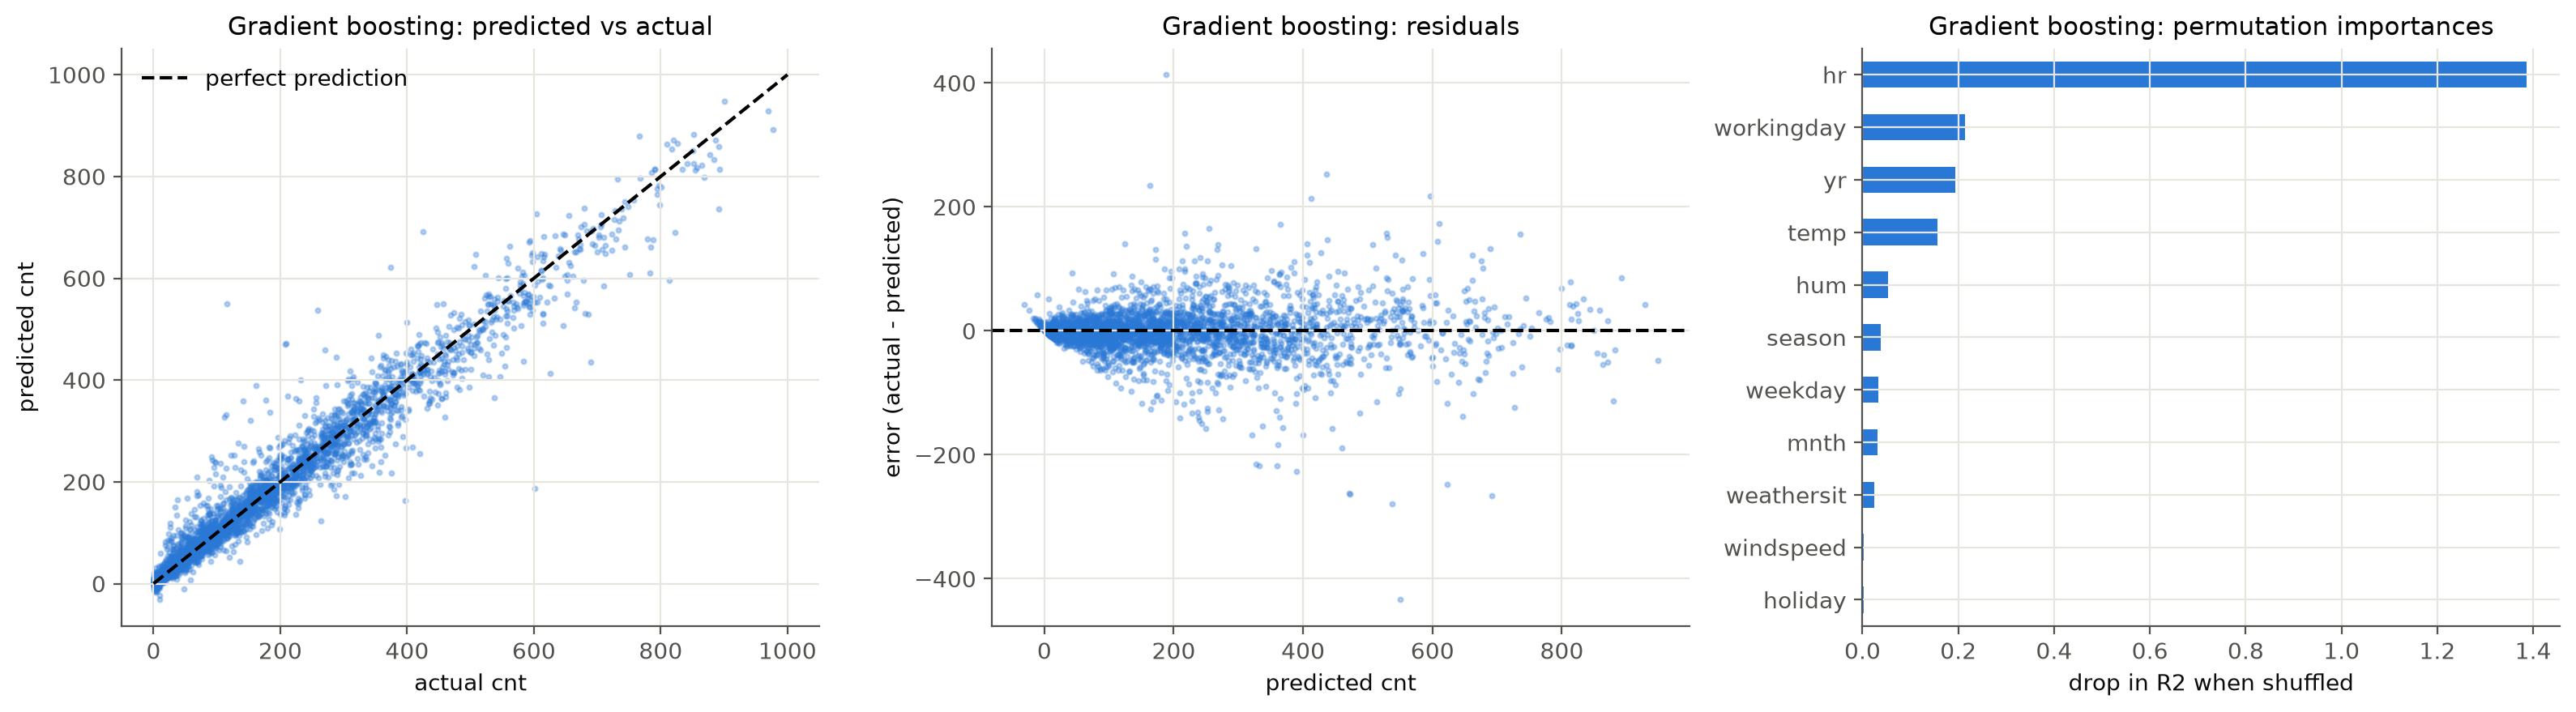
\includegraphics[width=\linewidth]{hgb.png}
  \caption{Gradient boosting: predicted vs actual, residuals, and permutation importance on the test set.}
  \label{fig:hgb}
\end{figure}

\textbf{Results.}
\begin{itemize}
  \item \textbf{Test:} RMSE 38.5, MAE 23.3, $R^2 = 0.953$, better than the random forest (42.0).
        \textbf{Train:} RMSE 27.4, so the train--test gap is 11 bikes against 26 for the forest: less overfitting.
  \item \textbf{Loss curve} (Figure~\ref{fig:hgbloss}): both losses fall quickly at first; after about 50 iterations
        the validation loss levels off (932 at iteration 50, 778 at the end) while the training loss keeps falling
        (656 to 330). The best validation loss was at iteration 183, and early stopping halted training at 193 of 500.
        The loss is half the squared error, so 778 corresponds to an RMSE of about 39 bikes, consistent with the test score.
  \item \textbf{Permutation importance} (drop in test $R^2$ when a feature is shuffled): \code{hr} 1.39, \code{workingday} 0.21,
        \code{yr} 0.19, \code{temp} 0.16; \code{windspeed} and \code{holiday} near 0. \code{workingday} ranks much higher than in the
        forest, consistent with the hour $\times$ working-day interaction. A drop above 1 is possible because $R^2$
        becomes negative when the model is badly wrong.
  \item \textbf{Limitation:} 50 test hours receive a negative prediction (minimum $-31.7$); clipping at 0 or a log target would fix this.
\end{itemize}

\subsection{Hyperparameter tuning}

Grid search tries every combination; random search samples combinations and is preferred for large
spaces. The space below has $4 \times 4 \times 3 \times 4 = 192$ combinations, of which random search
tried 20, each scored by \textbf{5-fold cross-validation} on the training set (the test set was not used).
\code{early\_stopping=True} was set explicitly so every candidate is regularized the same way.

\begin{table}[H]
\centering
\caption{Gradient boosting search space and selected values.}
\label{tab:tuning}
\small
\begin{tabularx}{\linewidth}{@{}l l c X@{}}
\toprule
Hyperparameter & Candidates & Selected & Effect \\
\midrule
\code{learning\_rate}     & 0.03, 0.05, 0.1, 0.2 & 0.03 & Contribution of each new tree. \\
\code{max\_leaf\_nodes}   & 15, 31, 63, 127      & 127  & Complexity of each tree. \\
\code{min\_samples\_leaf} & 10, 20, 50           & 10   & Minimum rows per leaf; larger values smooth predictions. \\
\code{l2\_regularization} & 0, 0.1, 1, 10        & 10   & L2 penalty on leaf values (the tree analogue of Ridge's $\lambda$). \\
\bottomrule
\end{tabularx}
\end{table}

\textbf{Results.} Best cross-validation RMSE 39.7; test RMSE 38.0, MAE 22.5, $R^2 = 0.954$ (vs 38.5, 23.3
and 0.953 untuned), an improvement of about 1\%. The five best settings all lie within 39.7--39.9, so the
model is insensitive to these hyperparameters and the remaining error is not a tuning problem. The
selected settings combine large, flexible trees with strong control (early stopping and L2 penalty).

% ===========================================================================
\section{Experimental Analysis}
% ===========================================================================

\textbf{Rationale.} The improved models were compared with learning curves (bias vs variance),
hour-by-hour predictions, and a stricter time-based split that tests performance on an unseen future period.

\subsection{Learning curves}

\begin{figure}[H]
  \centering
  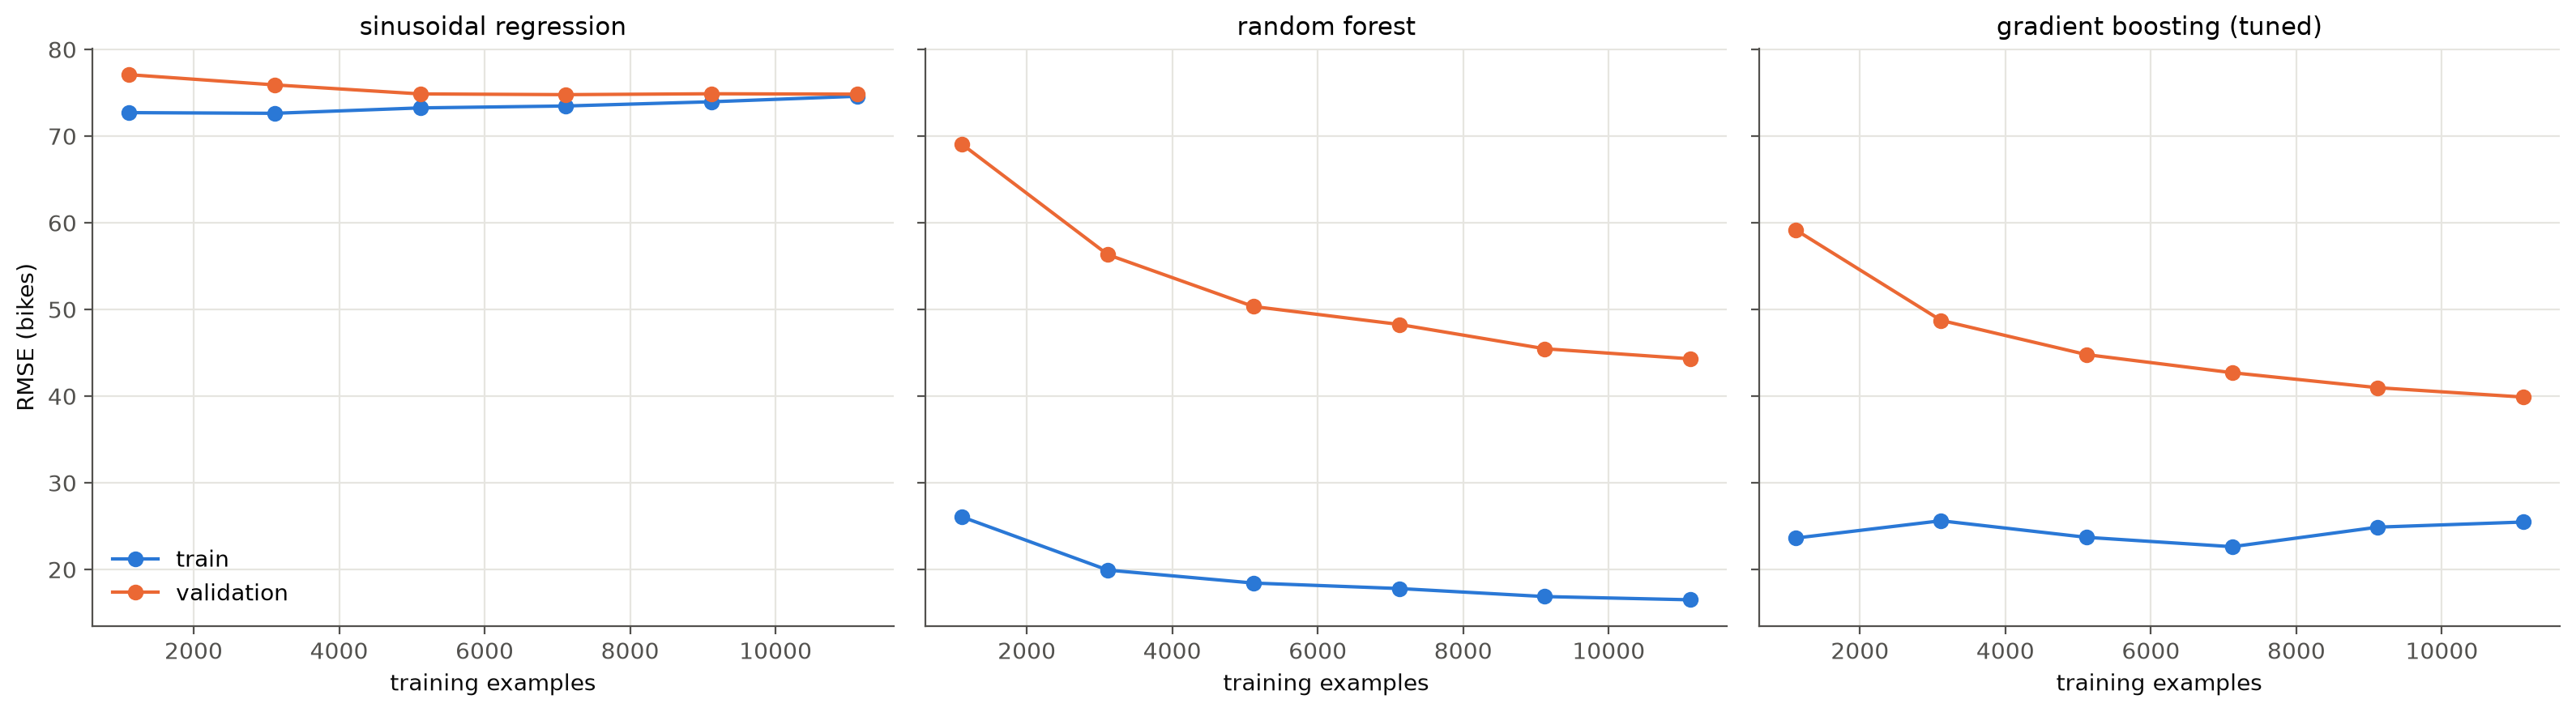
\includegraphics[width=\linewidth]{lc_all.png}
  \caption{Learning curves (5-fold cross-validation) for the sinusoidal model, random forest and tuned gradient boosting.}
  \label{fig:lcall}
\end{figure}

\begin{itemize}
  \item \textbf{Sinusoidal regression:} the curves converge at about 75 (74.6 train, 74.8 validation). Still
        \textbf{high bias}, but at half the baseline's plateau (142): better features lowered the plateau, and
        more data will not help further.
  \item \textbf{Random forest:} a large gap (16.5 train, 44.3 validation) with the validation error still
        falling: \textbf{high variance}; more data would still help.
  \item \textbf{Gradient boosting (tuned):} the lowest validation error (39.9), still falling slowly, with a
        smaller gap (training about 25.5) than the forest, because early stopping and L2 regularization limit variance.
\end{itemize}

\subsection{Two weeks of predictions}

\begin{figure}[H]
  \centering
  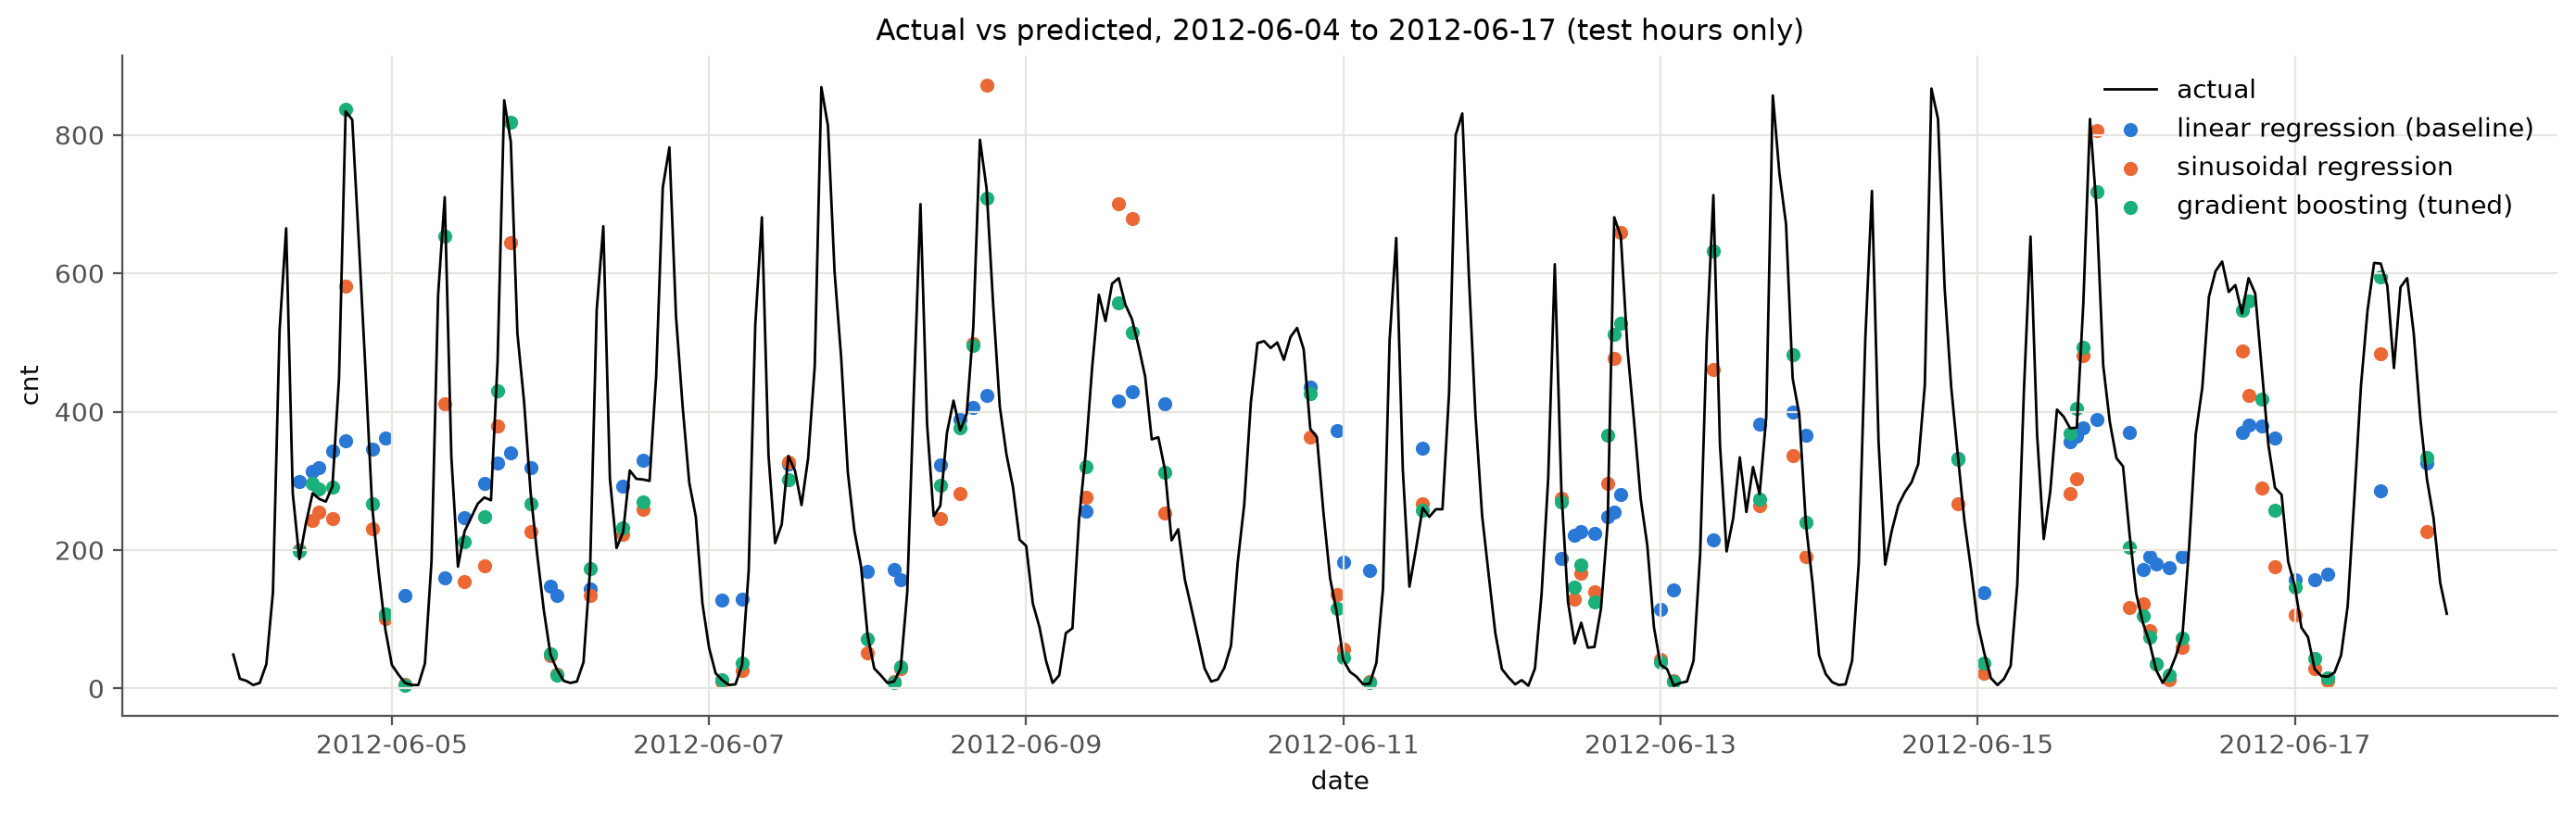
\includegraphics[width=\linewidth]{two_weeks.png}
  \caption{Actual hourly rentals (line) and predictions for the test hours from 4 to 17 June 2012.}
  \label{fig:twoweeks}
\end{figure}

The actual series shows two sharp peaks on each working day and a single rounded hump on the weekend
of 9--10 June. The linear baseline stays in a narrow band and misses every peak and trough; the
sinusoidal model follows the daily shape but undershoots several peaks; gradient boosting lands close
to the actual values at both peaks and troughs.

\subsection{Time-based split}

The random split treats hours as i.i.d., but neighbouring hours of the same day are very similar, so
the random test set is not fully unseen. Since a deployed model predicts the future, every model was
retrained with the same settings on the first 80\% of hours (1 January 2011 to 7 August 2012) and tested
on the last 20\% (7 August to 31 December 2012).

\begin{table}[H]
\centering
\caption{Test results on the random split and the time-based split. Best values in bold.}
\label{tab:results}
\small
\begin{tabular}{@{}lcccccc@{}}
\toprule
 & \multicolumn{3}{c}{Random split} & \multicolumn{3}{c}{Time split} \\
\cmidrule(lr){2-4}\cmidrule(lr){5-7}
Model & RMSE & MAE & $R^2$ & RMSE & MAE & $R^2$ \\
\midrule
Linear regression (baseline)         & 139.3 & 104.8 & 0.387 & 183.5 & 138.6 & 0.307 \\
Polynomial degree 4 + Ridge ($\lambda=100$) & 102.2 & 71.9 & 0.670 & 286.2 & 205.3 & $-0.684$ \\
Sinusoidal regression ($K=5$)        & 75.1  & 43.8  & 0.822 & 78.5  & 50.0  & 0.873 \\
Random forest                        & 42.0  & 24.6  & 0.944 & 70.1  & 45.4  & 0.899 \\
Gradient boosting                    & 38.5  & 23.3  & 0.953 & \textbf{64.8} & 42.4 & \textbf{0.914} \\
Gradient boosting (tuned)            & \textbf{38.0} & \textbf{22.5} & \textbf{0.954} & 65.5 & \textbf{42.3} & 0.912 \\
\bottomrule
\end{tabular}
\end{table}

\begin{figure}[H]
  \centering
  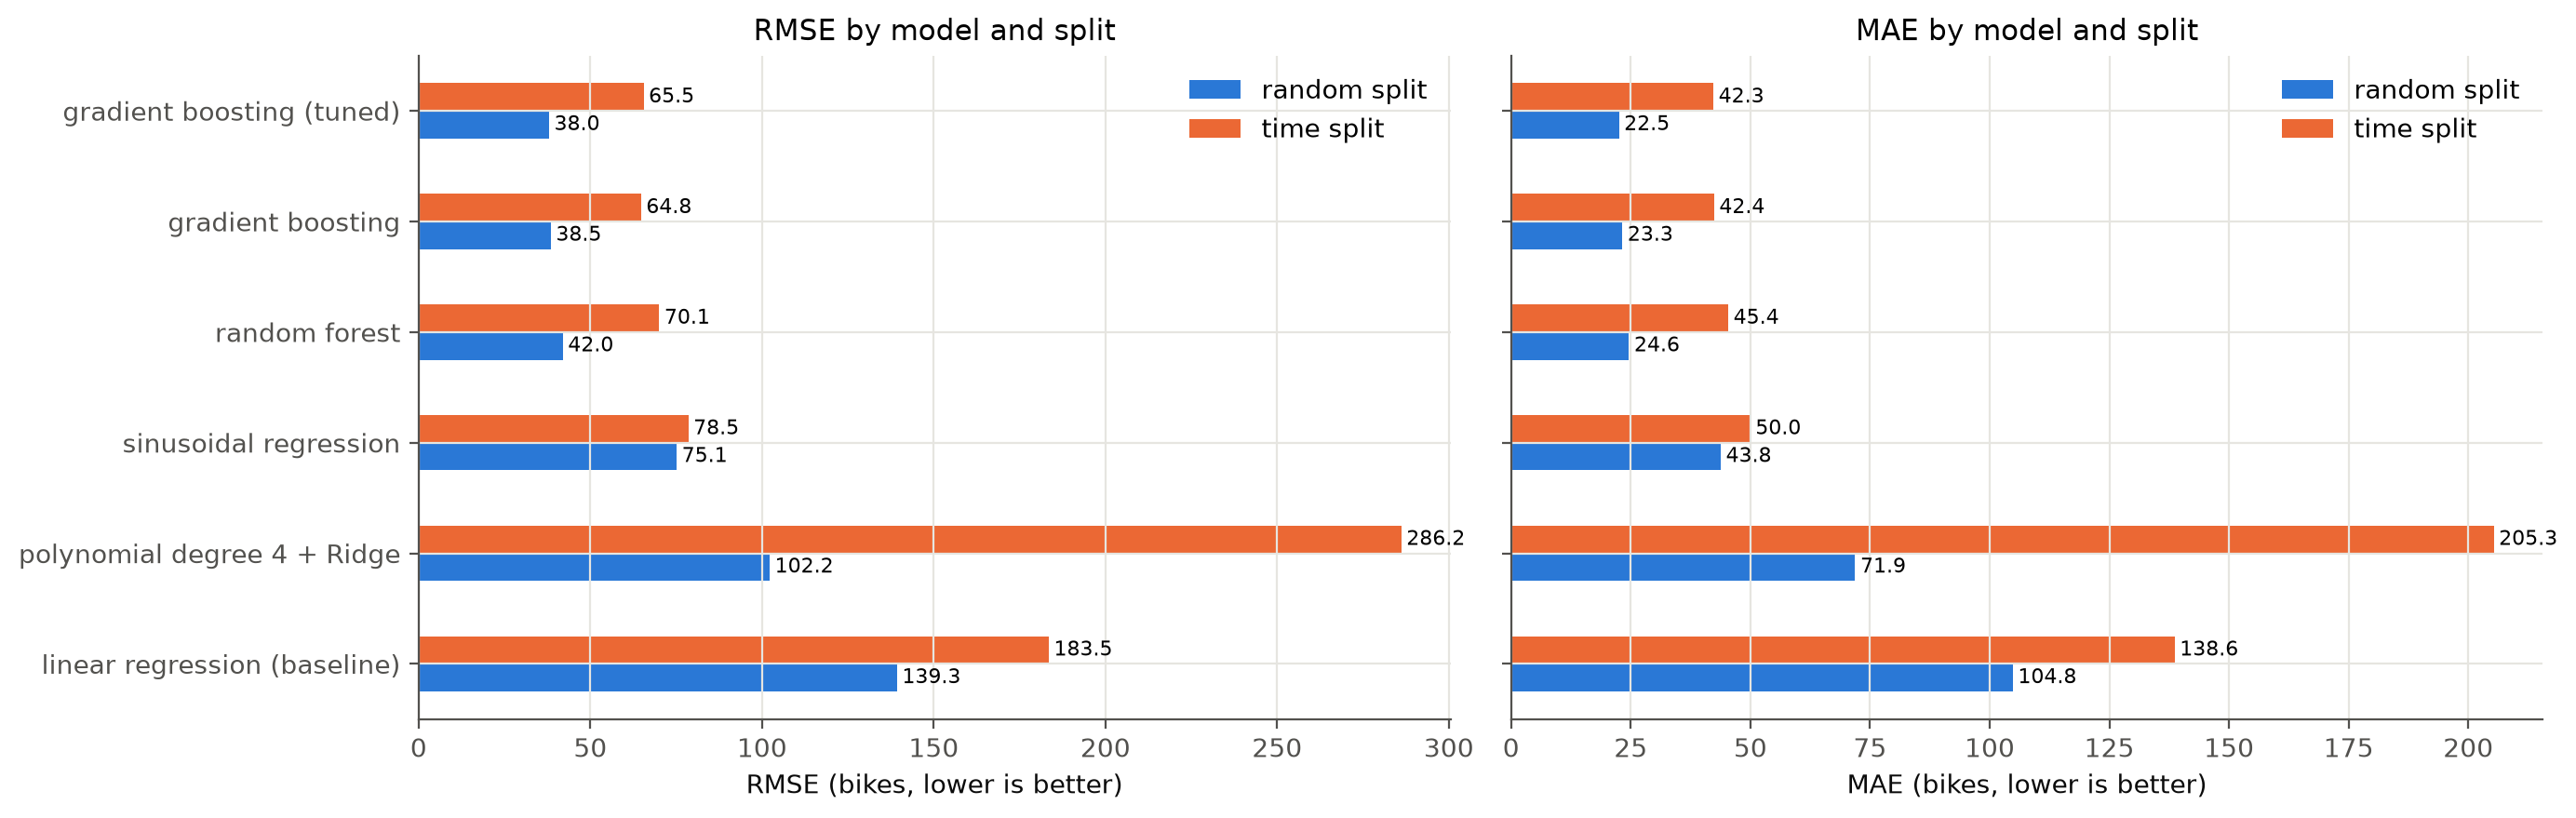
\includegraphics[width=\linewidth]{results.png}
  \caption{RMSE and MAE of every model on both splits (lower is better).}
  \label{fig:results}
\end{figure}

\subsection{Interpretation}

\begin{itemize}
  \item \textbf{Every model beats the baseline on the random split,} and gradient boosting is best on both
        splits. Tuned and untuned versions are within one bike of each other, so the tuning gain is not reliable.
  \item \textbf{All models get worse on the time split, by very different amounts:} RMSE rises 32\% for the
        baseline, 67\% for the random forest, 68\% for gradient boosting, and only about 5\% for the sinusoidal
        model. The random-split scores were optimistic, especially for trees, which benefit from having seen
        neighbouring hours of the same day.
  \item \textbf{The Ridge polynomial model collapses} ($R^2 = -0.684$, worse than predicting the mean). For
        November it predicts 90 bikes per hour on average against 213 actual, and 702 predictions are negative.
        The training period contains no ``2012 and November'' combination, so degree-4 terms such as
        $\text{yr}\times\text{mnth}^3$ \textbf{extrapolate} wildly. Regularization reduces variance within the
        range of the training data, but cannot fix extrapolation outside it.
  \item \textbf{The sinusoidal model generalizes best relative to its random-split score:} periodic features
        repeat rather than shoot off.
  \item \textbf{$R^2$ can mislead across test sets.} The sinusoidal model's $R^2$ rises (0.822 to 0.873) while its
        RMSE grows (75.1 to 78.5), because the time-split test period has more variance (standard deviation 220.5 vs
        178.0). RMSE and MAE are the fairer comparison.
  \item \textbf{MAE is much lower than RMSE for every model:} a small number of large errors, mostly at peak hours,
        account for much of the squared error.
\end{itemize}

% ===========================================================================
\section{Conclusions}
% ===========================================================================

\subsection{Main findings}

\begin{enumerate}
  \item \textbf{The hour of day is the key feature, and its effect depends on the type of day}: commute peaks
        on working days, a midday hump on weekends. Every successful model captured this non-linearity and interaction.
  \item \textbf{The linear baseline underfits} ($R^2 = 0.387$, RMSE 139.3). Equal train and test errors and a
        flat learning curve indicate high bias, not a lack of data. Gradient descent and the normal equation reach
        the same solution, so the model, not the optimizer, is the limit.
  \item \textbf{Increasing complexity exposes the bias--variance tradeoff}: polynomial features help up to degree 3,
        but degree 4 overfits (validation RMSE 425, weights up to 3,207). Tree depth shows the same tradeoff, with
        bagging keeping the forest's test error stable.
  \item \textbf{Regularization and feature engineering both improve the linear model}: Ridge ($\lambda=100$) gives RMSE
        102.2; five sine/cosine pairs with a working-day interaction and a log target give RMSE 75.1 with 31 columns.
  \item \textbf{Gradient boosting with early stopping is the best model} (RMSE 38.5, $R^2 = 0.953$; tuned 38.0),
        with less overfitting than the random forest.
  \item \textbf{The random split is optimistic for forecasting}: on a time-based split, tree-model errors grow by
        about 67\% and the Ridge polynomial collapses, while the sinusoidal model barely changes. Gradient boosting
        remains best (RMSE 64.8).
\end{enumerate}

\subsection{What worked and what did not}

\textbf{Worked:} starting from a simple baseline and diagnosing every model with training vs validation
error and learning curves, which pointed to the right remedy each time (more flexibility for high bias,
regularization for high variance); designing features from the exploration; controlling overfitting with
Ridge, early stopping and L2 penalties; choosing every hyperparameter on validation data or by
cross-validation, never on the test set; and testing on a time-based split.

\textbf{Did not work:}
\begin{itemize}
  \item Generic polynomial features: many columns, rapid overfitting, negative predictions, and poor extrapolation.
  \item More sine/cosine pairs beyond $K=5$: no further improvement.
  \item Hyperparameter tuning: about 1\% gain on the random split, slightly worse on the time split.
  \item Two further models were tried and dropped. Linear regression with one-hot encoded hours ($R^2 = 0.682$)
        still adds effects, so it has no hour $\times$ working-day interaction, and it gave 321 negative predictions.
        Periodic spline regression with interactions scored $R^2 = 0.922$ on the random split but $-5.67$ on the
        time split, predicting up to 3,421 bikes in an hour because its month $\times$ year interactions extrapolated.
\end{itemize}

\subsection{What I learned}

\begin{itemize}
  \item \textbf{Diagnose before improving:} whether a model suffers from bias or variance decides the next step.
  \item \textbf{Better features can beat more features:} 31 designed columns outperformed 1,364 polynomial ones.
  \item \textbf{How a model is evaluated matters as much as which model is chosen:} treating hours as i.i.d.\
        inflated every score, and only the time split revealed the extrapolation failures.
  \item \textbf{$R^2$ is not comparable across test sets} with different variance.
\end{itemize}

\subsection{Limitations and future work}

\begin{itemize}
  \item Lag features (previous hour, same hour yesterday) would suit next-hour forecasting; a quick test raised
        the random forest from $R^2 = 0.944$ to 0.960, but this changes the task.
  \item Clip negative predictions, or train gradient boosting on a log target.
  \item Use time-series cross-validation (\code{TimeSeriesSplit}) so that tuning also respects time order.
  \item Try L1 (Lasso) or Elastic Net to see which polynomial terms matter.
  \item In the linear models, categorical codes such as \code{weekday} are still treated as numbers.
\end{itemize}

% ===========================================================================
\begin{thebibliography}{9}
% ===========================================================================

\bibitem{uci}
H.~Fanaee-T. \emph{Bike Sharing} [Dataset]. UCI Machine Learning Repository, 2013.
\url{https://doi.org/10.24432/C5W894}

\bibitem{fanaee}
H.~Fanaee-T and J.~Gama. Event labeling combining ensemble detectors and background knowledge.
\emph{Progress in Artificial Intelligence}, 2(2--3):113--127, 2014.

\bibitem{sklearn}
F.~Pedregosa et al. Scikit-learn: Machine learning in Python.
\emph{Journal of Machine Learning Research}, 12:2825--2830, 2011.

\bibitem{geron}
A.~G\'eron. \emph{Hands-On Machine Learning with Scikit-Learn, Keras, and TensorFlow}, 3rd ed. O'Reilly Media, 2022.

\bibitem{lectures}
L.~Seyyed-Kalantari. CSSD 3131 lecture notes: Lectures 3, 5--9 (linear algebra, calculus,
regression I and II, overfitting and underfitting, regularization). York University, 2026.

\end{thebibliography}

\end{document}
